\documentclass[letterpaper,12pt,leqno]{report}

% Căn lề chuẩn
\usepackage[letterpaper, top=2.5cm, bottom=2.5cm, left=3cm, right=2cm]{geometry}

% Cấu hình Tiếng Việt và Font chữ
\usepackage[T5]{fontenc}
\usepackage[utf8]{inputenc}
\usepackage[vietnamese]{babel}
\usepackage{mathptmx}

% Các gói bảng, toán học và giao diện
\usepackage{array, booktabs, longtable}
\usepackage{amsmath, amsfonts, amssymb}
\usepackage{xcolor}
\usepackage{listings}
\usepackage[most]{tcolorbox}
\usepackage{enumitem}
\usepackage{indentfirst}
\usepackage{hyperref}

% Cấu hình
\usepackage{tocloft}
\renewcommand{\cftchappresnum}{Chương }
\setlength{\cftchapnumwidth}{5.5em}

\addto\captionsvietnamese{
  \renewcommand{\chaptername}{Chương}
  \renewcommand{\contentsname}{MỤC LỤC}
}

\hypersetup{
    colorlinks=true,
    linkcolor=blue,
    filecolor=magenta,      
    urlcolor=cyan,
    pdftitle={Bao cao Bai tap lon CSDL}
}

\begin{document}

% Trang bìa
\begin{titlepage}
    \centering
    \Large\textbf{TRƯỜNG ĐẠI HỌC GIAO THÔNG VẬN TẢI}\\[0.3cm]
    \Large\textbf{PHÂN HIỆU TẠI TP. HỒ CHÍ MINH}\\[1.5cm]

    \Huge\textbf{BÁO CÁO BÀI TẬP LỚN}\\[0.5cm]
    \Large\textbf{MÔN: THIẾT KẾ CƠ SỞ DỮ LIỆU}\\[1.5cm]

    \Large\textbf{Đề tài: Thiết kế Cơ sở Dữ liệu cho Hệ thống Giám sát và Bảo trì}\\[0.3cm]
    \Large\textbf{Cơ sở Hạ tầng Tích hợp Thực tế Tăng cường (AR-IMMS)}\\[0.3cm]

    \vfill
    \Large\textbf{TP. Hồ Chí Minh, Năm 2026}
\end{titlepage}

\cleardoublepage
\pagenumbering{arabic}

% Mục lục
\tableofcontents
\cleardoublepage

% phần mở đầu
\addtocontents{toc}{\protect\vspace{1em}\protect\noindent\textbf{\Large PHẦN MỞ ĐẦU}\par}

\chapter*{Lời mở đầu}
\pagestyle{plain}
\enlargethispage{3\baselineskip}
\addcontentsline{toc}{chapter}{Lời mở đầu}

\section*{1. Tính cấp thiết của Đề tài}
Trong các trung tâm dữ liệu (Data Center) và phòng máy chủ, việc quản lý và giám sát thiết bị phần cứng đóng vai trò rất quan trọng. Tuy nhiên, các dữ liệu giám sát (CPU/RAM, trạng thái máy chủ, lịch sử bảo trì) thường bị tách rời khỏi vị trí vật lý thực tế. Khi xảy ra sự cố, kỹ thuật viên gặp khó khăn trong việc xác định chính xác máy chủ bị lỗi giữa các tủ Rack, gây tốn thời gian xử lý.

Sự kết hợp giữa công nghệ \textbf{Thực tế Tăng cường (AR)} và \textbf{Cơ sở dữ liệu tập trung} cho phép gắn kết dữ liệu vận hành trực tiếp lên thiết bị thực tế qua mã QR/ArUco Marker. Để hệ thống AR và Web Admin truy xuất dữ liệu nhất quán, việc xây dựng một Cơ sở Dữ liệu (CSDL) chuẩn hóa là bước nền tảng cốt lõi.

Nhận thức được điều đó, nhóm chúng em đã lựa chọn đề tài: \textbf{“Thiết kế Cơ sở Dữ liệu cho Hệ thống Giám sát và Bảo trì Cơ sở Hạ tầng Tích hợp Thực tế Tăng cường (AR-IMMS)”} làm nội dung nghiên cứu cho bài tập lớn môn học.

\section*{2. Mục tiêu và Nội dung Thực hiện}
Đề tài tập trung áp dụng các kiến thức môn Thiết kế Cơ sở Dữ liệu để giải quyết bài toán quản lý dữ liệu cho hệ thống AR-IMMS với các mục tiêu chính:
\begin{itemize}
    \item \textbf{Phân tích \& Mô hình hóa Nghiệp vụ:} Khảo sát dòng chảy dữ liệu quản lý hạ tầng phòng máy (Site $\rightarrow$ Room $\rightarrow$ Rack $\rightarrow$ Server $\rightarrow$ Workload), quản lý cảnh báo, sự cố và phiếu bảo trì (ticket).
    \item \textbf{Thiết kế Mô hình CSDL chuẩn hóa:} Xây dựng sơ đồ thực thể liên kết (ERD), chuyển sang mô hình quan hệ và thực hiện chuẩn hóa dữ liệu đạt dạng chuẩn 3NF nhằm triệt tiêu dư thừa.
    \item \textbf{Cài đặt SQL \& Truy vấn dữ liệu:} Viết câu lệnh DDL khởi tạo CSDL, DML thao tác dữ liệu và ứng dụng Đại số quan hệ để tối ưu các truy vấn báo cáo.
\end{itemize}

\textbf{Phạm vi đề tài:} Thực hiện thiết kế CSDL ở các mức Quan niệm, Logic và Vật lý phục vụ mô hình thử nghiệm Mini Data Center trong khuôn khổ bài tập lớn môn học.

\vspace{0.4em}
Mặc dù đã cố gắng áp dụng kiến thức môn học để hoàn thiện báo cáo, song do hạn chế về kinh nghiệm thực tế, bài làm khó tránh khỏi những thiếu sót. Chúng em rất mong nhận được góp ý quý báu từ Thầy/Cô để đề tài được hoàn thiện hơn.

\vspace{0.4em}
\begin{raggedleft}
\textit{Chúng em xin chân thành cảm ơn!}\\
\end{raggedleft}

% phần nội dung chính
\addtocontents{toc}{\protect\vspace{1em}\protect\noindent\textbf{\Large PHẦN NỘI DUNG CHÍNH}\par}

\chapter{Khảo sát Yêu cầu \& Nghiệp vụ Hệ thống}
\chapter{Khảo sát Yêu cầu \& Nghiệp vụ Hệ thống}

\section{Mục tiêu và Phạm vi Khảo sát}

\subsection{Bối cảnh và Lý do khảo sát}
Trong bối cảnh chuyển đổi số, việc quản lý hạ tầng kỹ thuật tại các trung tâm dữ liệu đang chuyển dịch từ phương thức truyền thống sang các hệ thống giám sát hiện đại. Tuy nhiên, thực tế khảo sát cho thấy một rào cản lớn là sự tách rời giữa dữ liệu giám sát số và vị trí vật lý của thiết bị, khiến kỹ thuật viên mất nhiều thời gian để xác định vị trí lỗi trong thực tế. Do đó, việc khảo sát hệ thống là bước đi tiên quyết để nắm bắt dòng nghiệp vụ, từ đó thiết kế một giải pháp tích hợp Thực tế tăng cường (AR), mã nhận diện không gian và Cặp song sinh số (Digital Twin) nhằm tối ưu hóa hiệu quả vận hành.

\subsection{Mục tiêu khảo sát}
Quá trình khảo sát được thực hiện nhằm đạt được các mục tiêu cụ thể phục vụ cho giai đoạn thiết kế:
\begin{itemize}[leftmargin=2em]
    \item \textbf{Nắm vững dòng nghiệp vụ thực tế:} Phân tích quy trình từ lúc hệ thống thu thập chỉ số telemetry, phát hiện bất thường cho đến khi tạo sự cố và giao phiếu bảo trì cho kỹ thuật viên xử lý.
    \item \textbf{Xác định yêu cầu dữ liệu:} Đánh giá các tập dữ liệu đầu vào (thông tin phần cứng máy chủ, tủ Rack, chỉ số Telemetry) và dữ liệu đầu ra (nhật ký bảo trì, trạng thái vận hành).
    \item \textbf{Xây dựng các quy tắc nghiệp vụ:} Thu thập các ràng buộc về cấp độ ưu tiên của sự cố, quy trình phê duyệt khép kín phiếu công tác và mô hình phân quyền người dùng (RBAC).
    \item \textbf{Làm cơ sở thiết kế CSDL:} Tạo tiền đề để xây dựng mô hình thực thể liên kết (ERD) và chuẩn hóa dữ liệu, đảm bảo hệ thống vận hành ổn định.
\end{itemize}

\subsection{Phạm vi khảo sát}
Để đảm bảo tính khả thi trong phạm vi thiết kế, hoạt động khảo sát tập trung vào các phương diện trọng tâm sau:
\begin{itemize}[leftmargin=2em]
    \item \textbf{Đối tượng khảo sát:} Bao gồm hạ tầng phần cứng (Site, Room, Rack, Server) và các nhóm người dùng tương tác với hệ thống (Administrator, Operator, Field Technician).
    \item \textbf{Dữ liệu vận hành:} Tập trung vào các chỉ số thời gian thực như CPU, RAM, thông lượng mạng và trạng thái của các khối lượng công việc (Workload/Container).
    \item \textbf{Phân hệ chức năng:} Khảo sát sâu 4 phân hệ chính: Quản lý hạ tầng \& tài sản, Giám sát Telemetry \& Cảnh báo, Quản lý sự cố \& Phiếu bảo trì, và Quản trị an toàn hệ thống.
\end{itemize}

\subsection{Phương pháp thực hiện}
Việc thu thập thông tin được thực hiện chủ yếu thông qua \textbf{Phương pháp khảo sát tài liệu}. Nhóm tập trung nghiên cứu các quy trình vận hành chuẩn (SOP), tài liệu hướng dẫn thiết bị và các biểu mẫu báo cáo sự cố hiện có để xây dựng nền tảng lý thuyết và thực tiễn cho bản thiết kế.

\section{Nghiệp vụ Quản lý Hạ tầng và Workload}
Hạ tầng của hệ thống AR-IMMS được tổ chức theo mô hình cây phân cấp nghiêm ngặt nhằm liên kết chính xác không gian vật lý của Mini Data Center với tài sản kỹ thuật số.

\subsection{Cấu trúc Cây Phân cấp Hạ tầng}
Hệ thống tổ chức dữ liệu theo chuỗi quan hệ phụ thuộc $1:N$
\begin{equation*}
\text{Site} \longrightarrow \text{Room} \longrightarrow \text{Rack} \longrightarrow \text{Server} \longrightarrow \text{Workload}
\end{equation*}

\begin{itemize}[leftmargin=2em]
    \item \textbf{Trung tâm Dữ liệu (Site):} Đại diện cho địa điểm triển khai Mini Data Center, quản lý thông tin định danh \texttt{site\_id}, tên trung tâm \texttt{site\_name}, địa chỉ vị trí \texttt{location} và mô tả \texttt{description}.
    \item \textbf{Phòng Máy chủ (Room):} Không gian chứa các tủ Rack thuộc một Site. Mỗi Room lưu trữ \texttt{room\_id}, tên phòng \texttt{room\_name} và vị trí tầng \texttt{floor\_level}. Một Site chứa nhiều Room (\texttt{site\_id} là FK).
    \item \textbf{Tủ Rack (Rack):} Đơn vị lưu trữ đặt trong Room, định danh bởi \texttt{rack\_id}, \texttt{rack\_name}, sức chứa tối đa \texttt{max\_unit} và tọa độ \texttt{location\_in\_room}. Một Room chứa nhiều Rack (\texttt{room\_id} là FK).
    \item \textbf{Máy chủ Vật lý / Node (Server):} Thiết bị phần cứng lắp đặt tại vị trí U (\texttt{u\_position}) trong tủ Rack. Mỗi máy chủ lưu trữ \texttt{server\_id}, tên node \texttt{server\_name}, \texttt{ip\_address}, mã nhãn tài sản \texttt{asset\_tag}, số \texttt{serial\_number}, thông số cấu hình (\texttt{cpu\_model}, \texttt{ram\_total\_gb}, \texttt{storage\_total\_gb}), hạn bảo hành (\texttt{warranty}) và trạng thái vận hành \texttt{status}. Một Rack chứa nhiều Server (\texttt{rack\_id} là FK).
    \item \textbf{Khối lượng Công việc (Workload):} Các tiến trình hoặc ứng dụng dạng Docker Container chạy trên máy chủ, quản lý các thông tin \texttt{workload\_id}, \texttt{workload\_name}, \texttt{container\_id}, loại dịch vụ \texttt{service\_type} và trạng thái \texttt{status}. Một Server thực thi nhiều Workload (\texttt{server\_id} là FK).
\end{itemize}

\subsection{Nghiệp vụ Tương tác AR và Mã không gian}
\begin{itemize}[leftmargin=2em]
    \item Mỗi Server vật lý được gán một mã nhận diện không gian \texttt{qr\_code\_stamp} (dạng QR Code hoặc ArUco Marker) trực tiếp trên khung máy.
    \item Khi Kỹ thuật viên dùng ứng dụng Mobile AR quét mã \texttt{qr\_code\_stamp}, ứng dụng gửi truy vấn tra cứu thiết bị và hiển thị thông tin trực tiếp dạng phủ hình ảnh (AR Overlay).
\end{itemize}

% Phuong
\section{Nghiệp vụ Giám sát Vận hành và Quản lý Cảnh báo}
Phân hệ đảm nhận chức năng tiếp nhận chuỗi dữ liệu thời gian thực (real-time streaming telemetry) từ các lightweight collector agent, tự động đánh giá vi phạm ngưỡng và quản lý vòng đời cảnh báo.

\subsection{Thu thập Dữ liệu Đo lường Chuỗi thời gian}
\begin{itemize}[leftmargin=2em]
    \item Collector Agent cài đặt tại từng máy chủ tự động gửi dữ liệu định kỳ (mặc định \textbf{5 giây/lần}) lưu trữ vào thực thể \texttt{telemetry\_metric}.
    \item Mỗi bản ghi telemetry (\texttt{metric\_id}) gắn liền với một máy chủ (\texttt{server\_id}) bao gồm: tỷ lệ CPU (\texttt{cpu\_usage}), bộ nhớ RAM (\texttt{ram\_usage}), thông lượng mạng (\texttt{network\_traffic}), trạng thái các container (\texttt{container\_states}) dạng JSON và mốc thời gian \texttt{timestamp}.
    \item \textbf{Phát hiện mất kết nối:} Hệ thống cập nhật trường \texttt{last\_seen} trong thực thể \texttt{server}. Nếu quá \textbf{90 giây} không nhận được dữ liệu, trạng thái \texttt{status} của máy chủ tự động chuyển sang \texttt{unavailable}.
\end{itemize}

\subsection{Cấu hình Ngưỡng và Vòng đời Cảnh báo}
\begin{itemize}[leftmargin=2em]
    \item \textbf{Cấu hình ngưỡng (\texttt{alert\_threshold}):} Định nghĩa luật vi phạm cho từng loại chỉ số \texttt{metric\_type}, quy định mức cảnh báo nhẹ \texttt{warning\_value} và mức nguy hiểm \texttt{critical\_value}.
    \item \textbf{Phát sinh cảnh báo (\texttt{alert}):} Khi dữ liệu telemetry vượt ngưỡng hoặc kết nối bị ngắt, một sự kiện cảnh báo \texttt{alert\_id} tự động phát sinh liên kết với \texttt{server\_id} và \texttt{threshold\_id}.
    \item \textbf{Vòng đời xử lý Cảnh báo (\texttt{state}):} Cảnh báo được theo dõi qua các trạng thái:
    \begin{equation*}
    \text{\texttt{OPEN}} \longrightarrow \text{\texttt{ACKNOWLEDGED}} \longrightarrow \text{\texttt{RESOLVED}} \longrightarrow \text{\texttt{CLOSED}}
    \end{equation*}
    \item \textbf{Chống bão cảnh báo (Alert Suppression):} Nếu máy chủ đang bị sự cố và đã có phiếu xử lý \texttt{IN\_PROGRESS}, các cảnh báo trùng lặp tiếp theo sẽ tự động được gộp vào sự cố hiện tại.
\end{itemize}

\section{Nghiệp vụ Sự cố và Quản lý Phiếu Bảo trì}
Quy trình quản lý phiếu bảo trì khép kín luồng xử lý bằng cách chuyển hóa các cảnh báo tự động thành hành động thực địa của Kỹ thuật viên.

\subsection{Quản lý Sự cố và Lập Phiếu Bảo trì}
\begin{itemize}[leftmargin=2em]
    \item \textbf{Sự cố (\texttt{Incident}):} Khi cảnh báo chuyển sang trạng thái \texttt{ACKNOWLEDGED}, Người vận hành (Operator) tạo một \texttt{Incident} gom nhóm một hoặc nhiều cảnh báo gốc (\texttt{Alert}) liên quan, thiết lập độ nghiêm trọng \texttt{Severity} (\texttt{LOW}, \texttt{MEDIUM}, \texttt{HIGH}, \texttt{CRITICAL}).
    \item \textbf{Phiếu bảo trì (\texttt{MaintenanceTicket}):} Từ \texttt{Incident}, Operator lập các phiếu \texttt{MaintenanceTicket} giao việc cho Kỹ thuật viên (\texttt{AssignedTo}). Phiếu xác định rõ thiết bị mục tiêu \texttt{TargetID} (\texttt{SERVER}, \texttt{RACK}, \texttt{CONTAINER}), độ ưu tiên \texttt{Priority} và hạn chót \texttt{ScheduledAt}.
\end{itemize}

\subsection{Thực thi Bảo trì Hiện trường và Ghi Nhật ký}
\begin{itemize}[leftmargin=2em]
    \item \textbf{Tiến trình xử lý Phiếu bảo trì:} Phiếu công việc tuân thủ máy trạng thái:
    \begin{equation*}
    \text{\texttt{ASSIGNED}} \longrightarrow \text{\texttt{IN\_PROGRESS}} \longrightarrow \text{\texttt{PENDING\_APPROVAL}} \longrightarrow \text{\texttt{CLOSED}}
    \end{equation*}
    \item Kỹ thuật viên quét mã \texttt{QRCodeStamp} trên máy chủ bằng ứng dụng Mobile AR để tra cứu các phiếu bảo trì đang hoạt động (\texttt{ASSIGNED} / \texttt{IN\_PROGRESS}) gán cho thiết bị đó.
    \item \textbf{Nhật ký bảo trì (\texttt{MaintenanceLog}):} Khi thao tác, Kỹ thuật viên cập nhật nhật ký lưu lại cờ xác nhận có dùng AR (\texttt{ARSessionUsed}), ghi chú chẩn đoán (\texttt{InvestigationNotes}), nguyên nhân gốc (\texttt{RootCause}), biện pháp khắc phục (\texttt{CorrectiveAction}) và linh kiện thay thế (\texttt{PartsReplaced}).
    \item \textbf{Quy tắc phê duyệt đóng phiếu:} Kỹ thuật viên không được tự đóng ticket. Sau khi xử lý xong, Kỹ thuật viên chuyển ticket sang \texttt{PENDING\_APPROVAL}. Chỉ Operator mới có quyền phê duyệt đóng phiếu (\texttt{CLOSED}) và cập nhật trạng thái sự cố \texttt{Incident} sang \texttt{RESOLVED}/\texttt{CLOSED}.
\end{itemize}

% Hiệu
\section{Yêu cầu Hệ thống}
Dựa trên kết quả khảo sát nghiệp vụ ở các mục trước, phần này tổng hợp và phân loại các yêu cầu hệ thống cho nền tảng AR-IMMS thành hai nhóm chính: \textbf{Yêu cầu chức năng} (Functional Requirements) và \textbf{Yêu cầu phi chức năng} (Non-Functional Requirements). Các yêu cầu này là cơ sở trực tiếp để xác định các thực thể dữ liệu, quan hệ và ràng buộc trong thiết kế Cơ sở Dữ liệu ở các chương tiếp theo.

%% =============================================
%% 1.5.1 YÊU CẦU CHỨC NĂNG
%% =============================================
\subsection{Yêu cầu chức năng}
Hệ thống AR-IMMS phục vụ bốn nhóm tác nhân chính: \textit{Quản trị viên Hệ thống} (System Administrator), \textit{Vận hành viên} (System Operator), \textit{Kỹ thuật viên} (Technician) và \textit{Hệ thống Giám sát \& Cảnh báo Tự động} (Automated Monitoring \& Alerting System). Dưới đây là danh sách yêu cầu chức năng phân theo từng vai trò.

% ---- 1.5.1.1 Quản trị viên Hệ thống ----
\subsubsection{Quản trị viên Hệ thống (System Administrator)}
\begin{enumerate}[label=\textbf{FA-\arabic*}., leftmargin=2.5em]
    \item \textbf{Quản lý tài khoản người dùng:} Tạo mới, cập nhật thông tin, vô hiệu hóa và gán vai trò (Administrator, Operator, Technician) cho các tài khoản người dùng trên hệ thống.
    \item \textbf{Cấu hình thiết lập hệ thống:} Thiết lập và chỉnh sửa các thông số cấu hình toàn hệ thống (system-wide settings) bao gồm chu kỳ thu thập dữ liệu, ngưỡng cảnh báo mặc định, chính sách bảo mật và các tham số vận hành khác.
    \item \textbf{Giám sát tổng quan sức khỏe hệ thống:} Xem các chỉ số tổng hợp (aggregated indicators) về tình trạng hoạt động của toàn bộ hệ thống, bao gồm: tính khả dụng của dịch vụ (service availability), trạng thái kết nối của bộ thu thập dữ liệu (data collector connectivity) và lưu lượng cảnh báo (alert volume) trên tất cả các thành phần tích hợp.
    \item \textbf{Quản lý môi trường Mini Data Center:} Quản lý cấu hình các môi trường Mini Data Center thử nghiệm, bao gồm đăng ký site, phòng máy, và các thông số hệ thống liên quan.
    \item \textbf{Truy vấn nhật ký kiểm toán:} Xem và tra cứu nhật ký kiểm toán (audit log) ghi lại toàn bộ lịch sử thay đổi cấu hình, các hành động quản trị, và các sự kiện quan trọng trên hệ thống.
\end{enumerate}

% ---- 1.5.1.2 Vận hành viên ----
\subsubsection{Vận hành viên (System Operator)}
\begin{enumerate}[label=\textbf{FO-\arabic*}., leftmargin=2.5em]
    \item \textbf{Quản lý tài sản hạ tầng:} Đăng ký, cập nhật và quản lý thông tin các tủ Rack, máy chủ (Server/Node) và các khối tải công việc (Workload/Container) tương ứng theo hệ thống phân cấp: Site $\rightarrow$ Room $\rightarrow$ Rack $\rightarrow$ Node $\rightarrow$ Workload.
    \item \textbf{Liên kết mã đánh dấu không gian (Spatial Marker):} Gán mã định danh QR/ArUco Marker cho một máy chủ hoặc node đã đăng ký trong quá trình tiếp nhận thiết bị (onboarding). Cho phép cập nhật liên kết khi phần cứng được di chuyển hoặc thay thế.
    \item \textbf{Giám sát trạng thái vận hành:} Theo dõi trạng thái vận hành theo thời gian thực (real-time) và dữ liệu lịch sử (historical) của toàn bộ hạ tầng Mini Data Center, bao gồm mức sử dụng CPU, RAM, ổ đĩa, lưu lượng mạng và trạng thái container.
    \item \textbf{Tương tác Digital Twin:} Xem và tương tác với mô hình Digital Twin để nhận diện trạng thái, vị trí và mối quan hệ phân cấp giữa các tủ Rack, máy chủ và dịch vụ đang chạy.
    \item \textbf{Cấu hình ngưỡng cảnh báo:} Thiết lập các ngưỡng (threshold) cho từng chỉ số giám sát, rà soát các điều kiện bất thường và xác nhận (acknowledge) các cảnh báo đang hoạt động.
    \item \textbf{Quản lý sự cố và phiếu bảo trì:} Xác nhận cảnh báo đang hoạt động; khi cần xử lý, tạo phiếu sự cố (incident) hoặc phiếu bảo trì (maintenance ticket) tham chiếu đến cảnh báo gốc. Gán, theo dõi phiếu công việc, lập báo cáo vận hành và quản lý lịch sử dịch vụ.
    \item \textbf{Phân tích xu hướng và báo cáo:} Xem các báo cáo xu hướng lịch sử (historical trend reports), các chỉ số quy hoạch dung lượng (capacity planning metrics) và phân tích PUE/tiêu thụ điện năng, được nhóm theo site, phòng máy, tủ rack và node.
    \item \textbf{Quản lý thông số kỹ thuật thiết bị:} Ghi nhận và cập nhật thông số kỹ thuật phần cứng (hardware specifications), thông tin bảo hành (warranty) và lịch sử bảo trì (maintenance history) cho các tài sản đã đăng ký.
\end{enumerate}

% ---- 1.5.1.3 Kỹ thuật viên ----
\subsubsection{Kỹ thuật viên (Technician)}
\begin{enumerate}[label=\textbf{FT-\arabic*}., leftmargin=2.5em]
    \item \textbf{Tiếp nhận phiếu công việc:} Xem danh sách các phiếu sự cố hoặc phiếu bảo trì được giao, nhận diện tủ Rack và máy chủ cần kiểm tra.
    \item \textbf{Nhận diện thiết bị bằng AR:} Sử dụng ứng dụng AR trên thiết bị di động để quét mã QR/ArUco Marker gắn trên phần cứng, từ đó nhận diện thiết bị và truy cập thông tin vận hành theo ngữ cảnh (contextual operational information) được hiển thị trực tiếp trên hình ảnh camera.
    \item \textbf{Xem thông tin chi tiết thiết bị:} Truy cập trạng thái máy chủ, dữ liệu giám sát thời gian thực (telemetry), cảnh báo đang hoạt động, thông tin chẩn đoán (diagnostic information) và danh sách các workload/dịch vụ liên quan.
    \item \textbf{Cập nhật tiến trình xử lý:} Xác nhận tiếp nhận công việc, cập nhật trạng thái xử lý, ghi nhận ghi chú điều tra (investigation notes), nguyên nhân xác định (identified causes) và các biện pháp khắc phục (corrective actions).
    \item \textbf{Hoàn tất và đóng phiếu:} Ghi nhận kết quả bảo trì, xem lại lịch sử dịch vụ của thiết bị, đánh dấu sự cố đã giải quyết (resolved) và gửi yêu cầu đóng phiếu (ticket closure request) để Vận hành viên phê duyệt.
\end{enumerate}

% ---- 1.5.1.4 Hệ thống Giám sát & Cảnh báo Tự động ----
\subsubsection{Hệ thống Giám sát và Cảnh báo Tự động}
\begin{enumerate}[label=\textbf{FS-\arabic*}., leftmargin=2.5em]
    \item \textbf{Thu thập dữ liệu vận hành:} Tự động thu thập dữ liệu telemetry (CPU, RAM, ổ đĩa, mạng, Docker container) và trạng thái kết nối từ các máy chủ đã đăng ký theo chu kỳ được cấu hình.
    \item \textbf{Phát hiện bất thường:} Tự động phát hiện các máy chủ không khả dụng (unavailable), các luồng thu thập dữ liệu bị gián đoạn (interrupted data collection) và các chỉ số vận hành vượt ngưỡng đã cấu hình.
    \item \textbf{Quản lý vòng đời cảnh báo:} Tạo mới và cập nhật trạng thái cảnh báo xuyên suốt vòng đời: Mở (Open) $\rightarrow$ Đã xác nhận (Acknowledged) $\rightarrow$ Đã giải quyết (Resolved) $\rightarrow$ Đã đóng (Closed).
    \item \textbf{Lưu trữ dữ liệu lịch sử và kiểm toán:} Lưu trữ dữ liệu telemetry lịch sử vào cơ sở dữ liệu chuỗi thời gian (time-series database); ghi nhận các hoạt động giám sát, cảnh báo và bảo trì quan trọng vào nhật ký kiểm toán (audit log).
\end{enumerate}

% ---- Bảng tổng hợp yêu cầu chức năng ----
\vspace{0.5em}
\noindent\textbf{Bảng tổng hợp yêu cầu chức năng theo vai trò:}

\vspace{0.3em}
\begin{longtable}{|c|l|p{8.5cm}|}
\hline
\textbf{Mã} & \textbf{Vai trò} & \textbf{Yêu cầu chức năng} \\
\hline
\endfirsthead
\hline
\textbf{Mã} & \textbf{Vai trò} & \textbf{Yêu cầu chức năng} \\
\hline
\endhead
\hline
\endfoot
FA-1 & Administrator & Quản lý tài khoản người dùng (CRUD, gán vai trò) \\
\hline
FA-2 & Administrator & Cấu hình thiết lập toàn hệ thống \\
\hline
FA-3 & Administrator & Giám sát tổng quan sức khỏe hệ thống \\
\hline
FA-4 & Administrator & Quản lý môi trường Mini Data Center \\
\hline
FA-5 & Administrator & Truy vấn nhật ký kiểm toán \\
\hline
FO-1 & Operator & Quản lý tài sản hạ tầng (Rack, Node, Workload) \\
\hline
FO-2 & Operator & Liên kết mã đánh dấu không gian QR/ArUco \\
\hline
FO-3 & Operator & Giám sát trạng thái vận hành thời gian thực \& lịch sử \\
\hline
FO-4 & Operator & Tương tác Digital Twin \\
\hline
FO-5 & Operator & Cấu hình ngưỡng cảnh báo \\
\hline
FO-6 & Operator & Quản lý sự cố và phiếu bảo trì \\
\hline
FO-7 & Operator & Phân tích xu hướng và báo cáo vận hành \\
\hline
FO-8 & Operator & Quản lý thông số kỹ thuật \& bảo hành thiết bị \\
\hline
FT-1 & Technician & Tiếp nhận phiếu công việc được giao \\
\hline
FT-2 & Technician & Nhận diện thiết bị bằng AR (QR/ArUco scan) \\
\hline
FT-3 & Technician & Xem thông tin chi tiết thiết bị \& telemetry \\
\hline
FT-4 & Technician & Cập nhật tiến trình xử lý \\
\hline
FT-5 & Technician & Hoàn tất và đóng phiếu bảo trì \\
\hline
FS-1 & Hệ thống tự động & Thu thập dữ liệu vận hành theo chu kỳ \\
\hline
FS-2 & Hệ thống tự động & Phát hiện bất thường \& vượt ngưỡng \\
\hline
FS-3 & Hệ thống tự động & Quản lý vòng đời cảnh báo \\
\hline
FS-4 & Hệ thống tự động & Lưu trữ telemetry lịch sử \& nhật ký kiểm toán \\
\hline
\end{longtable}

%% =============================================
%% 1.5.2 YÊU CẦU PHI CHỨC NĂNG
%% =============================================
\subsection{Yêu cầu phi chức năng}
Bên cạnh các yêu cầu chức năng, hệ thống AR-IMMS cần đáp ứng các yêu cầu phi chức năng sau đây để đảm bảo chất lượng vận hành trong thực tiễn. Các yêu cầu phi chức năng này cũng ảnh hưởng trực tiếp đến việc thiết kế cấu trúc CSDL, lựa chọn kiểu dữ liệu, chiến lược đánh chỉ mục (indexing), và cơ chế phân vùng (partitioning).

% ---- 1.5.2.1 Hiệu năng (Performance) ----
\subsubsection{Hiệu năng (Performance)}
\begin{itemize}[leftmargin=2em]
    \item Dữ liệu telemetry từ các máy chủ phải được thu thập theo chu kỳ cấu hình được, với chu kỳ mặc định là \textbf{5 giây}.
    \item Một máy chủ sẽ được báo cáo là \textit{không khả dụng} (unavailable) khi không nhận được dữ liệu telemetry trong vòng hơn \textbf{90 giây}.
    \item Hệ thống phải hỗ trợ truyền phát dữ liệu theo thời gian thực qua WebSocket với độ trễ thấp, cho phép điều hướng drilldown liền mạch từ tổng quan đến chi tiết container trong tối đa 3 lần nhấp chuột.
\end{itemize}

% ---- 1.5.2.2 Khả dụng (Availability) ----
\subsubsection{Khả dụng (Availability)}
\begin{itemize}[leftmargin=2em]
    \item Nền tảng phải hoạt động ổn định trong các giờ làm việc dự kiến.
    \item Hệ thống phải thông báo cho người dùng khi một máy chủ hoặc bộ thu thập dữ liệu (data collector) trở nên không khả dụng.
    \item Các dịch vụ quan trọng (Backend API, WebSocket Gateway) cần được theo dõi tính khả dụng liên tục.
\end{itemize}

% ---- 1.5.2.3 Bảo mật (Security) ----
\subsubsection{Bảo mật (Security)}
\begin{itemize}[leftmargin=2em]
    \item Hệ thống phải thực thi xác thực (authentication) cho mọi truy cập và phân quyền dựa trên vai trò (Role-Based Access Control -- RBAC) với ba vai trò: Administrator, Operator và Technician.
    \item Sử dụng \textbf{JWT} (JSON Web Token) cho xác thực API và \textbf{mTLS} (mutual TLS) cho các kết nối từ telemetry agent đến backend.
    \item Tất cả các thay đổi cấu hình, cập nhật phiếu bảo trì và các hành động từ xa (remote actions) phải được ghi nhận vào nhật ký kiểm toán (audit log) với đầy đủ thông tin: người thực hiện, thời điểm, hành động, và đối tượng bị tác động.
\end{itemize}

% ---- 1.5.2.4 Độ tin cậy (Reliability) ----
\subsubsection{Độ tin cậy (Reliability)}
\begin{itemize}[leftmargin=2em]
    \item Các telemetry agent phải tự động thử lại (retry) khi truyền dữ liệu thất bại và tự phục hồi (resume) sau khi kết nối lại thành công.
    \item Hệ thống phải triệt tiêu cảnh báo trùng lặp (duplicate suppression) để ngăn chặn tình trạng bão cảnh báo (alert storm).
    \item Các sự cố phải tuân theo vòng đời trạng thái rõ ràng: Open $\rightarrow$ In-Progress $\rightarrow$ Resolved $\rightarrow$ Closed, được quản lý bằng máy trạng thái (state machine) trong CSDL.
\end{itemize}

% ---- 1.5.2.5 Khả năng mở rộng (Scalability) ----
\subsubsection{Khả năng mở rộng (Scalability)}
\begin{itemize}[leftmargin=2em]
    \item Bản PoC (Proof of Concept) phải chứng minh rằng một node xử lý mới được thêm vào sẽ bắt đầu truyền telemetry và xuất hiện trong Digital Twin trong vòng \textbf{5 phút} kể từ khi đăng ký.
    \item Việc thêm node mới chỉ yêu cầu cấu hình thông tin đăng nhập (credentials) và địa chỉ endpoint, \textbf{không} cần sửa đổi mã nguồn dịch vụ lõi (core service code).
    \item Cấu trúc CSDL phải hỗ trợ mở rộng theo chiều ngang (horizontal scalability) -- cho phép thêm nhiều site, room, rack và node mà không ảnh hưởng đến hiệu năng truy vấn.
\end{itemize}

% ---- 1.5.2.6 Khả năng sử dụng (Usability) ----
\subsubsection{Khả năng sử dụng (Usability)}
\begin{itemize}[leftmargin=2em]
    \item Hệ thống cung cấp giao diện dashboard \textbf{desktop-first} bằng tiếng Anh trên nền tảng Web (Next.js) và ứng dụng AR trên Android (React Native).
    \item Giao diện người dùng phải responsive, dễ tiếp cận (accessible), hiển thị rõ ràng trạng thái sức khỏe máy chủ, chi tiết sự cố, các bước khắc phục và hướng dẫn bảo trì.
    \item Hỗ trợ điều hướng phân cấp liền mạch: Site $\rightarrow$ Room $\rightarrow$ Rack $\rightarrow$ Node $\rightarrow$ Workload với giao diện drilldown trực quan.
\end{itemize}

% ---- 1.5.2.7 Bảo trì & An toàn (Maintainability & Safety) ----
\subsubsection{Bảo trì và An toàn (Maintainability \& Safety)}
\begin{itemize}[leftmargin=2em]
    \item Hệ thống phải hỗ trợ kiểm thử tự động (automated testing), ghi log tập trung (centralized logging), và cho phép cấu hình linh hoạt các chỉ số giám sát cùng ngưỡng cảnh báo.
    \item Các hành động có tính phá hủy hoặc ảnh hưởng lớn (ví dụ: khởi động lại dịch vụ từ phiên AR) phải yêu cầu \textbf{xác nhận} (confirmation) trước khi thực thi và được ghi vào nhật ký kiểm toán.
    \item Mã nguồn backend và frontend phải được tổ chức theo kiến trúc module, hỗ trợ triển khai bằng container (containerized deployment) để thuận tiện cho việc bảo trì và nâng cấp.
\end{itemize}

% ---- Bảng tổng hợp yêu cầu phi chức năng ----
\vspace{0.5em}
\noindent\textbf{Bảng tổng hợp yêu cầu phi chức năng:}

\vspace{0.3em}
\begin{longtable}{|c|p{3cm}|p{9cm}|}
\hline
\textbf{Mã} & \textbf{Thuộc tính} & \textbf{Mô tả yêu cầu} \\
\hline
\endfirsthead
\hline
\textbf{Mã} & \textbf{Thuộc tính} & \textbf{Mô tả yêu cầu} \\
\hline
\endhead
\hline
\endfoot
NF-1 & Hiệu năng & Thu thập telemetry mặc định 5s; phát hiện unavailable sau 90s \\
\hline
NF-2 & Hiệu năng & Truyền phát real-time qua WebSocket, drilldown $\leq$ 3 click \\
\hline
NF-3 & Khả dụng & Hoạt động ổn định giờ làm việc; thông báo khi server/collector unavailable \\
\hline
NF-4 & Bảo mật & Xác thực JWT, phân quyền RBAC (3 vai trò), mTLS cho agent \\
\hline
NF-5 & Bảo mật & Audit log đầy đủ cho mọi thay đổi cấu hình và hành động quan trọng \\
\hline
NF-6 & Độ tin cậy & Agent tự retry/resume; triệt tiêu cảnh báo trùng lặp \\
\hline
NF-7 & Độ tin cậy & Vòng đời sự cố: Open $\rightarrow$ In-Progress $\rightarrow$ Resolved $\rightarrow$ Closed \\
\hline
NF-8 & Khả năng mở rộng & Node mới streaming telemetry $\leq$ 5 phút; không sửa mã nguồn lõi \\
\hline
NF-9 & Khả năng sử dụng & Dashboard desktop-first (Web), AR app (Android); giao diện responsive \\
\hline
NF-10 & Bảo trì \& An toàn & Automated testing, centralized logging; xác nhận trước hành động phá hủy \\
\hline
\end{longtable}

%% =============================================
%% 1.5.3 ÁNH XẠ YÊU CẦU VÀO ĐỐI TƯỢNG DỮ LIỆU
%% =============================================
\subsection{Ánh xạ Yêu cầu vào Đối tượng Dữ liệu chính}
Từ các yêu cầu chức năng và phi chức năng trên, có thể nhận diện các nhóm đối tượng dữ liệu chính mà CSDL của hệ thống AR-IMMS cần quản lý. Bảng dưới đây tóm tắt ánh xạ từ yêu cầu sang các thực thể dữ liệu trọng yếu, làm cơ sở cho việc xây dựng mô hình ERD ở Chương 2.

\vspace{0.3em}
\begin{longtable}{|p{3.5cm}|p{4cm}|p{6cm}|}
\hline
\textbf{Nhóm yêu cầu} & \textbf{Đối tượng dữ liệu} & \textbf{Mô tả} \\
\hline
\endfirsthead
\hline
\textbf{Nhóm yêu cầu} & \textbf{Đối tượng dữ liệu} & \textbf{Mô tả} \\
\hline
\endhead
\hline
\endfoot
Quản lý tài khoản, phân quyền (FA-1, NF-4) & User, Role & Tài khoản người dùng, vai trò RBAC, token xác thực \\
\hline
Quản lý tài sản hạ tầng (FO-1, FO-2, FO-8) & Site, Room, Rack, Node, Workload, SpatialMarker & Hệ thống phân cấp tài sản, thông số kỹ thuật, mã marker \\
\hline
Thu thập \& giám sát (FO-3, FS-1, NF-1) & TelemetryRecord, CollectorStatus & Dữ liệu telemetry chuỗi thời gian, trạng thái kết nối agent \\
\hline
Cảnh báo (FO-5, FS-2, FS-3, NF-6, NF-7) & Alert, AlertThreshold & Ngưỡng cảnh báo, cảnh báo với vòng đời trạng thái \\
\hline
Sự cố \& phiếu bảo trì (FO-6, FT-1 -- FT-5) & Incident, Ticket, TicketActivity & Phiếu sự cố, phiếu bảo trì, ghi chú xử lý, lịch sử dịch vụ \\
\hline
Bảo hành \& lịch sử bảo trì (FO-8) & Warranty, MaintenanceLog & Thông tin bảo hành, lịch sử bảo trì thiết bị \\
\hline
Kiểm toán (FA-5, NF-5, FS-4) & AuditLog & Nhật ký kiểm toán ghi lại mọi thay đổi quan trọng \\
\hline
Báo cáo \& phân tích (FO-7, NF-2) & Report, TrendAnalytics & Báo cáo vận hành, phân tích xu hướng, PUE metrics \\
\hline
Cấu hình hệ thống (FA-2, FA-4) & SystemConfig, DataCenterConfig & Tham số cấu hình hệ thống, thiết lập môi trường DC \\
\hline
\end{longtable}

\vspace{0.3em}
\noindent Các đối tượng dữ liệu được xác định ở trên sẽ được phân tích chi tiết, xác định thuộc tính, mối quan hệ và ràng buộc toàn vẹn trong \textbf{Chương 2 -- Thiết kế Mô hình Dữ liệu quan niệm} và tiếp tục được chuẩn hóa trong \textbf{Chương 3 -- Thiết kế Mô hình Logic \& Chuẩn hóa}.



\chapter{Thiết kế Quan niệm (Mô hình ERD)}
\clearpage

\chapter{Thiết kế Mô hình Dữ liệu Quan niệm}

\section{Xác định Các Thực thể và Thuộc tính}

% Phuong
\section{Sơ đồ Thực thể Kết hợp (ERD)}

Dựa trên danh sách các thực thể, thuộc tính đã xác định và mô hình bài toán quản lý hạ tầng Mini Data Center, sơ đồ thực thể Kết hợp ERD được thiết lập nhằm thể hiện cấu trúc lưu trữ và các mối quan hệ giữa các phân hệ trong hệ thống.

\subsection{Danh sách các Mối quan hệ giữa các Thực thể}

Hệ thống bao gồm 16 mối quan hệ chính giữa các thực thể, đảm bảo tính toàn vẹn dữ liệu từ hạ tầng vật lý đến các tác vụ vận hành thực địa:

\begin{table}[H]
\centering
\caption{Bảng tổng hợp các mối quan hệ trong sơ đồ ERD}
\label{tab:erd_relationships}
\begin{tabular}{|c|l|c|l|p{4.5cm}|}
\hline
\textbf{STT} & \textbf{Thực thể A} & \textbf{Quan hệ (A : B)} & \textbf{Thực thể B} & \textbf{Ý nghĩa nghiệp vụ} \\ \hline
1 & Site & 1 : N & Room & Một trung tâm dữ liệu chứa nhiều phòng máy. \\ \hline
2 & Room & 1 : N & Rack & Một phòng máy chứa nhiều tủ Rack. \\ \hline
3 & Rack & 1 : N & Server & Một tủ Rack chứa nhiều máy chủ vật lý. \\ \hline
4 & Server & 1 : N & Workload & Một máy chủ chạy nhiều Workload/Container. \\ \hline
5 & Server & 1 : N & TelemetryMetric & Một máy chủ thu thập nhiều bản ghi đo lường thời gian thực. \\ \hline
6 & AlertThreshold & 1 : N & Alert & Một cấu hình ngưỡng có thể kích hoạt nhiều sự kiện cảnh báo. \\ \hline
7 & Server & 1 : N & Alert & Một máy chủ có thể phát sinh nhiều sự kiện cảnh báo. \\ \hline
8 & User & 1 : N & Alert & Một người dùng có thể xác nhận (\texttt{AcknowledgedBy}) nhiều cảnh báo. \\ \hline
9 & Alert & 1 : N & Incident & Một cảnh báo có thể leo thang thành nhiều sự cố. \\ \hline
10 & User & 1 : N & Incident & Một người dùng có thể khởi tạo (\texttt{CreatedBy}) nhiều sự cố. \\ \hline
11 & Server & 1 : N & MaintenanceTicket & Một máy chủ có thể liên quan tới nhiều phiếu bảo trì. \\ \hline
12 & Incident & 1 : N & MaintenanceTicket & Một sự cố có thể tạo ra nhiều phiếu bảo trì hiện trường. \\ \hline
13 & User & 1 : N & MaintenanceTicket & Người dùng phân công (\texttt{CreatedBy}) hoặc tiếp nhận (\texttt{AssignedTo}) phiếu. \\ \hline
14 & MaintenanceTicket & 1 : N & MaintenanceLog & Một phiếu bảo trì có nhiều nhật ký ghi nhận tiến độ. \\ \hline
15 & User & 1 : N & MaintenanceLog & Một kỹ thuật viên (\texttt{TechnicianID}) ghi lại nhiều nhật ký. \\ \hline
16 & Asset & 1 : N & MaintenanceLog & Một tài sản phần cứng có thể được thay thế/sửa chữa trong nhật ký. \\ \hline
17 & AssetCategory & 1 : N & Asset & Một danh mục quản lý nhiều tài sản phần cứng. \\ \hline
18 & Server & 1 : N & Asset & Một máy chủ có thể gắn nhiều linh kiện tài sản. \\ \hline
19 & Asset & 1 : N & Warranty & Một tài sản có thể có nhiều hợp đồng bảo hành theo thời gian. \\ \hline
20 & Asset & 1 : N & AssetStatusChange & Một tài sản lưu trữ nhiều lịch sử thay đổi trạng thái. \\ \hline
21 & User & 1 : N & UserRole & Một người dùng có thể đảm nhận nhiều vai trò. \\ \hline
22 & Role & 1 : N & UserRole & Một vai trò có thể được gán cho nhiều người dùng. \\ \hline
23 & User & 1 : N & AuditLog & Một người dùng thực hiện nhiều thao tác lưu trong nhật ký kiểm toán. \\ \hline
\end{tabular}
\end{table}

\subsection{Các Trục Liên kết Trung tâm}

Mô hình ERD được thiết kế tối ưu xoay quanh 2 trục dữ liệu cốt lõi:

\begin{itemize}[leftmargin=2em]
    \item \textbf{Trục hạ tầng phần cứng (\texttt{Server}):} Liên kết phân tầng từ vị trí địa lý ($\text{Site} \rightarrow \text{Room} \rightarrow \text{Rack} \rightarrow \text{Server}$) xuống các dịch vụ ảo hóa (\texttt{Workload}), đồng thời kết nối trực tiếp đến dữ liệu telemetry, cảnh báo, phiếu bảo trì và tài sản phần cứng thông qua khóa ngoại \texttt{ServerID}.
    \item \textbf{Trục vận hành \& định danh (\texttt{User}):} Đóng vai trò kiểm soát truy cập và dấu vết kiểm toán. \texttt{UserID} xuất hiện làm khóa ngoại tại các bảng \texttt{Alert} (người xác nhận), \texttt{Incident} (người tạo), \texttt{MaintenanceTicket} (người tạo / kỹ thuật viên), \texttt{MaintenanceLog} (kỹ thuật viên xử lý) và \texttt{AuditLog} (người thực hiện thao tác).
\end{itemize}

\subsection{Sơ đồ ERD Tổng quan Hệ thống}

Sơ đồ ERD thể hiện chi tiết danh sách thực thể, thuộc tính (khóa chính PK, khóa ngoại FK) cùng bản thể quan hệ (Cardinality) được trình bày như Hình \ref{fig:erd_diagram}.

\begin{figure}[H]
    \centering
    % Bạn hãy thay tên file ảnh sơ đồ vẽ được từ Draw.io / Lucidchart vào đây
    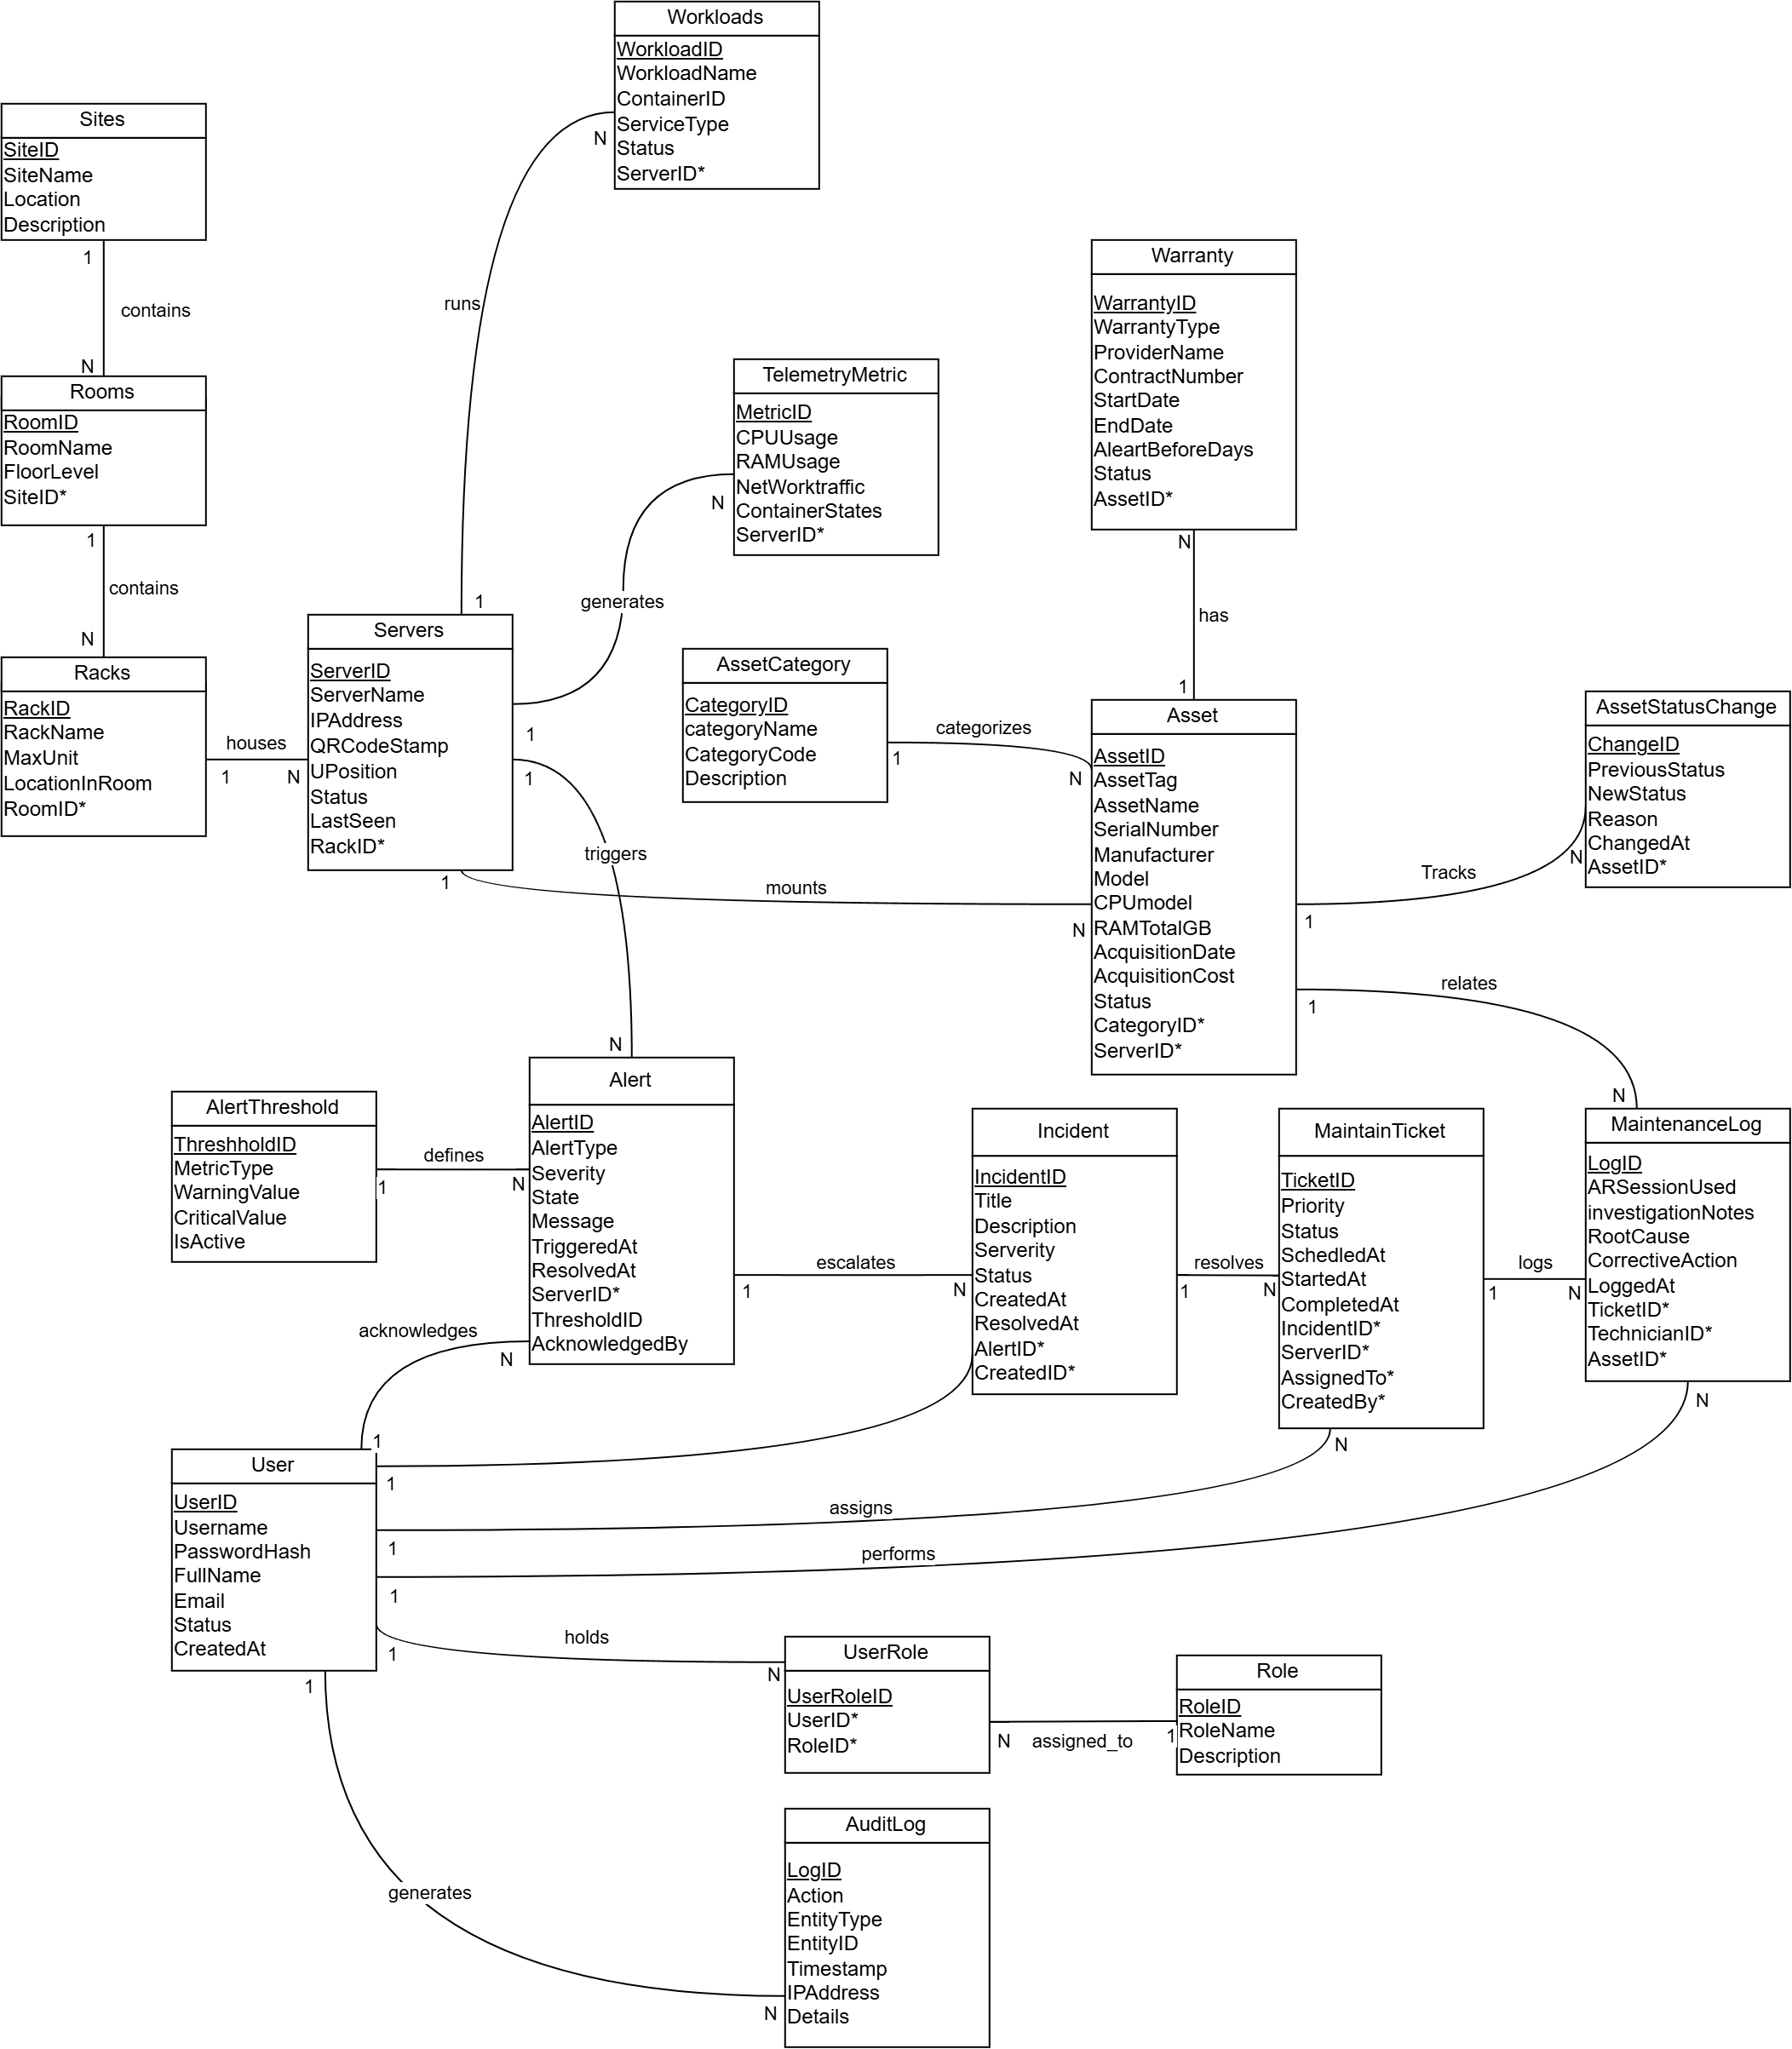
\includegraphics[width=1.0\textwidth]{images/erd_diagram.png} 
    \caption{Sơ đồ Thực thể Kết hợp (ERD) hệ thống Quản lý Mini Data Center}
    \label{fig:erd_diagram}
\end{figure}

% Ky Anh
\section{Các Quy tắc Nghiệp vụ (Business Rules)}

Để đảm bảo tính toàn vẹn dữ liệu, an toàn vận hành hạ tầng Mini Data Center và tính chính xác của các quy trình giám sát, hệ thống áp dụng các quy tắc nghiệp vụ và ràng buộc toàn vẹn cụ thể như sau:

\subsection{Ràng buộc Miền giá trị (Domain Constraints)}
\begin{itemize}[leftmargin=2em]
    \item \textbf{Cấu hình phần cứng \& Tải trọng:}
    \begin{itemize}
        \item Chiều cao tủ Rack (\texttt{Rack.MaxUnit}) và vị trí lắp đặt server (\texttt{Server.UPosition}) phải là các số nguyên dương ($> 0$).
        \item Tổng dung lượng RAM (\texttt{Asset.RAMTotalGB}) và dung lượng lưu trữ (\texttt{Asset.StorageTotalGB}) phải là số nguyên lớn hơn $0$.
    \end{itemize}
    \item \textbf{Chỉ số Telemetry \& Giám sát:}
    \begin{itemize}
        \item Mức độ sử dụng CPU (\texttt{TelemetryMetric.CPUUsage}) và RAM (\texttt{TelemetryMetric.RAMUsage}) phải nằm trong khoảng $[0, 100]\%$.
        \item Lưu lượng mạng (\texttt{TelemetryMetric.NetworkTraffic}) phải có giá trị không âm ($\ge 0$).
        \item Giá trị ngưỡng cảnh báo mức Nguy hiểm phải lớn hơn mức Cảnh báo (\texttt{AlertThreshold.CriticalValue} $>$ \texttt{AlertThreshold.WarningValue}).
    \end{itemize}
    \item \textbf{Định danh \& Tài khoản người dùng:}
    \begin{itemize}
        \item Email (\texttt{User.Email}) và Tên đăng nhập (\texttt{User.Username}) phải duy nhất (\texttt{UNIQUE}) trên toàn hệ thống và đúng định dạng chuẩn.
        \item Mã thẻ tài sản (\texttt{Asset.AssetTag}) và Số sê-ri (\texttt{Asset.SerialNumber}) phải là duy nhất (\texttt{UNIQUE}).
    \end{itemize}
\end{itemize}

\subsection{Ràng buộc Tham chiếu và Toàn vẹn Thực thể (Referential Integrity)}
\begin{itemize}[leftmargin=2em]
    \item \textbf{Phân cấp Hạ tầng vất lý:} 
    \begin{itemize}
        \item Một phòng máy (\texttt{Room}) bắt buộc phải thuộc một Trung tâm dữ liệu (\texttt{Site}) hợp lệ. Không cho phép xóa \texttt{Site} khi còn tồn tại các \texttt{Room} bên trong (\texttt{ON DELETE RESTRICT}).
        \item Máy chủ (\texttt{Server}) bắt buộc phải thuộc một tủ Rack (\texttt{Rack}) cụ thể.
    \end{itemize}
    \item \textbf{Chuỗi phát sinh Cảnh báo \& Sự cố:}
    \begin{itemize}
        \item Bản ghi cảnh báo (\texttt{Alert}) phải tham chiếu tới một máy chủ (\texttt{ServerID}) và một cấu hình ngưỡng (\texttt{ThresholdID}) đang hoạt động.
        \item Sự cố (\texttt{Incident}) chỉ được khởi tạo khi liên kết tới một \texttt{AlertID} hợp lệ hoặc do một tài khoản người dùng (\texttt{CreatedBy}) có thẩm quyền tạo trực tiếp.
        \item Phiếu bảo trì (\texttt{MaintenanceTicket}) phải được phân công cho một kỹ thuật viên (\texttt{AssignedTo}) tồn tại trong bảng \texttt{User}.
    \end{itemize}
\end{itemize}

\subsection{Ràng buộc Liên thuộc tính \& Logic Thời gian (Temporal \& Inter-attribute Constraints)}
\begin{itemize}[leftmargin=2em]
    \item \textbf{Vòng đời xử lý Cảnh báo \& Sự cố:}
    \begin{itemize}
        \item Thời điểm giải quyết cảnh báo phải sau thời điểm cảnh báo kích hoạt ($\text{Alert.ResolvedAt} \ge \text{Alert.TriggeredAt}$).
        \item Thời điểm khắc phục sự cố phải sau thời điểm ghi nhận sự cố ($\text{Incident.ResolvedAt} \ge \text{Incident.CreatedAt}$).
    \end{itemize}
    \item \textbf{Tiến độ Phiếu bảo trì (Maintenance Ticket):}
    \begin{itemize}
        \item Mốc thời gian thực hiện phiếu bảo trì phải tuân theo thứ tự tuyến tính: 
        \[
        \text{ScheduledAt} \le \text{StartedAt} \le \text{CompletedAt}
        \]
        \item Thời điểm ghi nhật ký bảo trì (\texttt{MaintenanceLog.LoggedAt}) không được sớm hơn thời điểm bắt đầu xử lý phiếu (\texttt{MaintenanceTicket.StartedAt}).
    \end{itemize}
    \item \textbf{Thời hạn Bảo hành Tài sản:}
    \begin{itemize}
        \item Ngày kết thúc hợp đồng bảo hành phải sau ngày bắt đầu hiệu lực ($\text{Warranty.EndDate} > \text{Warranty.StartDate}$).
        \item Ngày ghi nhận thay đổi trạng thái tài sản (\texttt{AssetStatusChange.ChangedAt}) phải lớn hơn hoặc bằng ngày mua sắm (\texttt{Asset.AcquisitionDate}).
    \end{itemize}
\end{itemize}

\subsection{Ràng buộc Nghiệp vụ Đơn động \& Phân quyền (Operational \& RBAC Rules)}
\begin{itemize}[leftmargin=2em]
    \item \textbf{Chuyển đổi trạng thái Máy chủ \& Cảnh báo:}
    \begin{itemize}
        \item Nếu máy chủ rơi vào trạng thái \textit{"Offline"} hoặc \textit{"Critical"}, hệ thống tự động ngắt trạng thái hoạt động của các \texttt{Workload} chạy trên máy chủ đó.
        \item Chỉ người dùng (\texttt{User}) có vai trò (\texttt{Role}) là \textit{"Operator"} hoặc \textit{"System Admin"} mới có quyền tiếp nhận (\texttt{AcknowledgedBy}) cảnh báo hoặc đóng sự cố (\texttt{Incident}).
    \end{itemize}
    \item \textbf{Kiểm toán vết hệ thống (Audit Trail):}
    \begin{itemize}
        \item Mọi thao tác thêm, sửa, xóa tài sản phần cứng (\texttt{Asset}), phân công phiếu bảo trì (\texttt{MaintenanceTicket}) hoặc thay đổi quyền hạn (\texttt{UserRole}) bắt buộc phải tự động kích hoạt ghi bản ghi mới vào nhật ký kiểm toán (\texttt{AuditLog}) với đầy đủ \texttt{UserID}, \texttt{Action}, \texttt{Timestamp} và \texttt{IPAddress}.
        \item Dữ liệu trong bảng \texttt{AuditLog} chỉ cho phép ghi mới (\texttt{INSERT}), tuyệt đối không cho phép chỉnh sửa (\texttt{UPDATE}) hoặc xóa (\texttt{DELETE}).
    \end{itemize}
\end{itemize}



\chapter{Thiết kế Logic \& Chuẩn hóa Dạng chuẩn}
\clearpage

\chapter{Thiết kế Mô hình Dữ liệu Logic và Cơ sở Vật lý}

%An
\section{Chuyển đổi từ Mô hình Quan niệm sang Lược đồ Logic}

Dựa trên sơ đồ thực thể kết nối (ERD) và các quy tắc nghiệp vụ đã phân tích ở chương trước, tiến hành chuyển đổi mô hình thực thể quan niệm sang mô hình quan hệ (Relational Schema). Quá trình này được thực hiện thông qua việc áp dụng nghiêm ngặt lý thuyết chuẩn hóa cơ sở dữ liệu (đảm bảo đạt tối thiểu chuẩn 3NF dựa trên tập phủ tối thiểu của các phụ thuộc hàm) nhằm loại bỏ hoàn toàn dư thừa dữ liệu, triệt tiêu các dị thường khi thêm, xóa, sửa, đồng thời đảm bảo tính toàn vẹn tham chiếu và tối ưu hóa hiệu năng truy vấn cho toàn bộ hệ thống quản lý hạ tầng Mini Data Center.

Quá trình chuyển đổi từ các thực thể, thuộc tính và mối quan hệ sang cấu trúc bảng quan hệ tuân thủ các nguyên tắc thiết kế hiện đại: sử dụng khóa chính dạng định danh duy nhất (UUID/$\text{VARCHAR}(36)$) cho toàn bộ các thực thể cốt lõi, áp dụng kiểu dữ liệu tối ưu cho từng loại thuộc tính ($\text{DATETIME}$, $\text{FLOAT}$, $\text{TEXT}$), chuẩn hóa quy tắc đặt tên theo chuẩn PascalCase, và thiết lập đầy đủ các ràng buộc khóa ngoại ($\text{FK}$) nhằm duy trì tính liên kết chặt chẽ giữa các bảng.

Các bảng dữ liệu trong hệ thống được phân rã, tổ chức và phân nhóm thành các phân hệ chức năng chi tiết sau:

\begin{itemize}[leftmargin=2em]
    \item \textbf{Phân hệ Hạ tầng \& Không gian Vật lý:} 
    Quản lý phân cấp không gian và thiết bị từ cấp độ vị trí trung tâm (\texttt{Site}), phòng máy chuyên dụng (\texttt{Room}), tủ chứa thiết bị (\texttt{Rack}) cho đến thiết bị máy chủ vật lý (\texttt{Server}) và các dịch vụ ảo hóa, container chạy trên nền tảng đó (\texttt{Workload}). Việc thiết kế chuỗi liên kết khóa ngoại từ $\text{Site} \to \text{Room} \to \text{Rack} \to \text{Server} \to \text{Workload}$ giúp ánh xạ chính xác sơ đồ vị trí và cấu trúc phân cấp vật lý thực tế vào mô hình dữ liệu quan hệ, hỗ trợ việc tra cứu và quản lý tài nguyên hạ tầng một cách trực quan.

    \item \textbf{Phân hệ Giám sát \& Vận hành Hệ thống:} 
    Chịu trách nhiệm lưu trữ chuỗi thời gian của các chỉ số hiệu năng phần cứng theo thời gian thực như mức độ sử dụng CPU, RAM, lưu lượng mạng và trạng thái container (\texttt{TelemetryMetric}). Đồng thời, phân hệ này quản lý việc thiết lập các ngưỡng cảnh báo động (\texttt{AlertThreshold}), ghi nhận các sự kiện cảnh báo phát sinh (\texttt{Alert}), sự cố hệ thống trầm trọng (\texttt{Incident}) và theo dõi toàn bộ vòng đời xử lý nghiệp vụ bảo trì từ khâu lập phiếu, phân công kỹ thuật viên cho đến khi hoàn tất (\texttt{MaintainTicket}, \texttt{MaintenanceLog}), kết hợp ghi nhận các phiên thao tác thực tế qua kính thực tế ảo tăng cường (\text{ARSessionUsed}).

    \item \textbf{Phân hệ Quản lý Tài sản \& Bảo hành:} 
    Quản lý toàn bộ vòng đời của thiết bị phần cứng thông qua danh mục phân loại tài sản (\texttt{AssetCategory}), bảng thông tin chi tiết tài sản liên kết với máy chủ hoặc thiết bị độc lập (\texttt{Asset}), theo dõi thông tin hợp đồng bảo hành với nhà cung cấp, thời hạn hiệu lực và cấu hình cảnh báo trước hạn (\texttt{Warranty}), cùng bảng ghi nhận lịch sử biến động trạng thái tài sản theo thời gian (\texttt{AssetStatusChange}) để phục vụ công tác kiểm kê và thanh lý.

    \item \textbf{Phân hệ Bảo mật, Phân quyền \& Kiểm toán:} 
    Đảm bảo tính an toàn, phân quyền truy cập chặt chẽ và khả năng truy vết hệ thống thông qua bảng quản lý thông tin tài khoản người dùng (\texttt{User}), định nghĩa các vai trò chức năng trong hệ thống (\texttt{Role}), bảng liên kết nhiều-nhiều quản lý phân quyền người dùng (\texttt{UserRole}) và cơ chế ghi vết nhật ký kiểm toán toàn cục (\texttt{AuditLog}) lưu lại mọi thao tác quan trọng kèm theo địa chỉ IP và mã thực thể tác động.
\end{itemize}

Thông qua quá trình chuẩn hóa và hiện thực hóa tường minh các mối quan hệ kết nối dạng một - nhiều ($1 - N$) từ sơ đồ ERD, mô hình quan hệ đã thiết lập một nền tảng vững chắc, đảm bảo tính nhất quán dữ liệu cao, sẵn sàng cho việc triển khai mã nguồn và xây dựng các câu lệnh truy vấn tối ưu ở các giai đoạn tiếp theo của đồ án.

\subsection{Sơ đồ Lược đồ Quan hệ (Relational Schema Diagram)}

\begin{figure}[H]
    \centering
    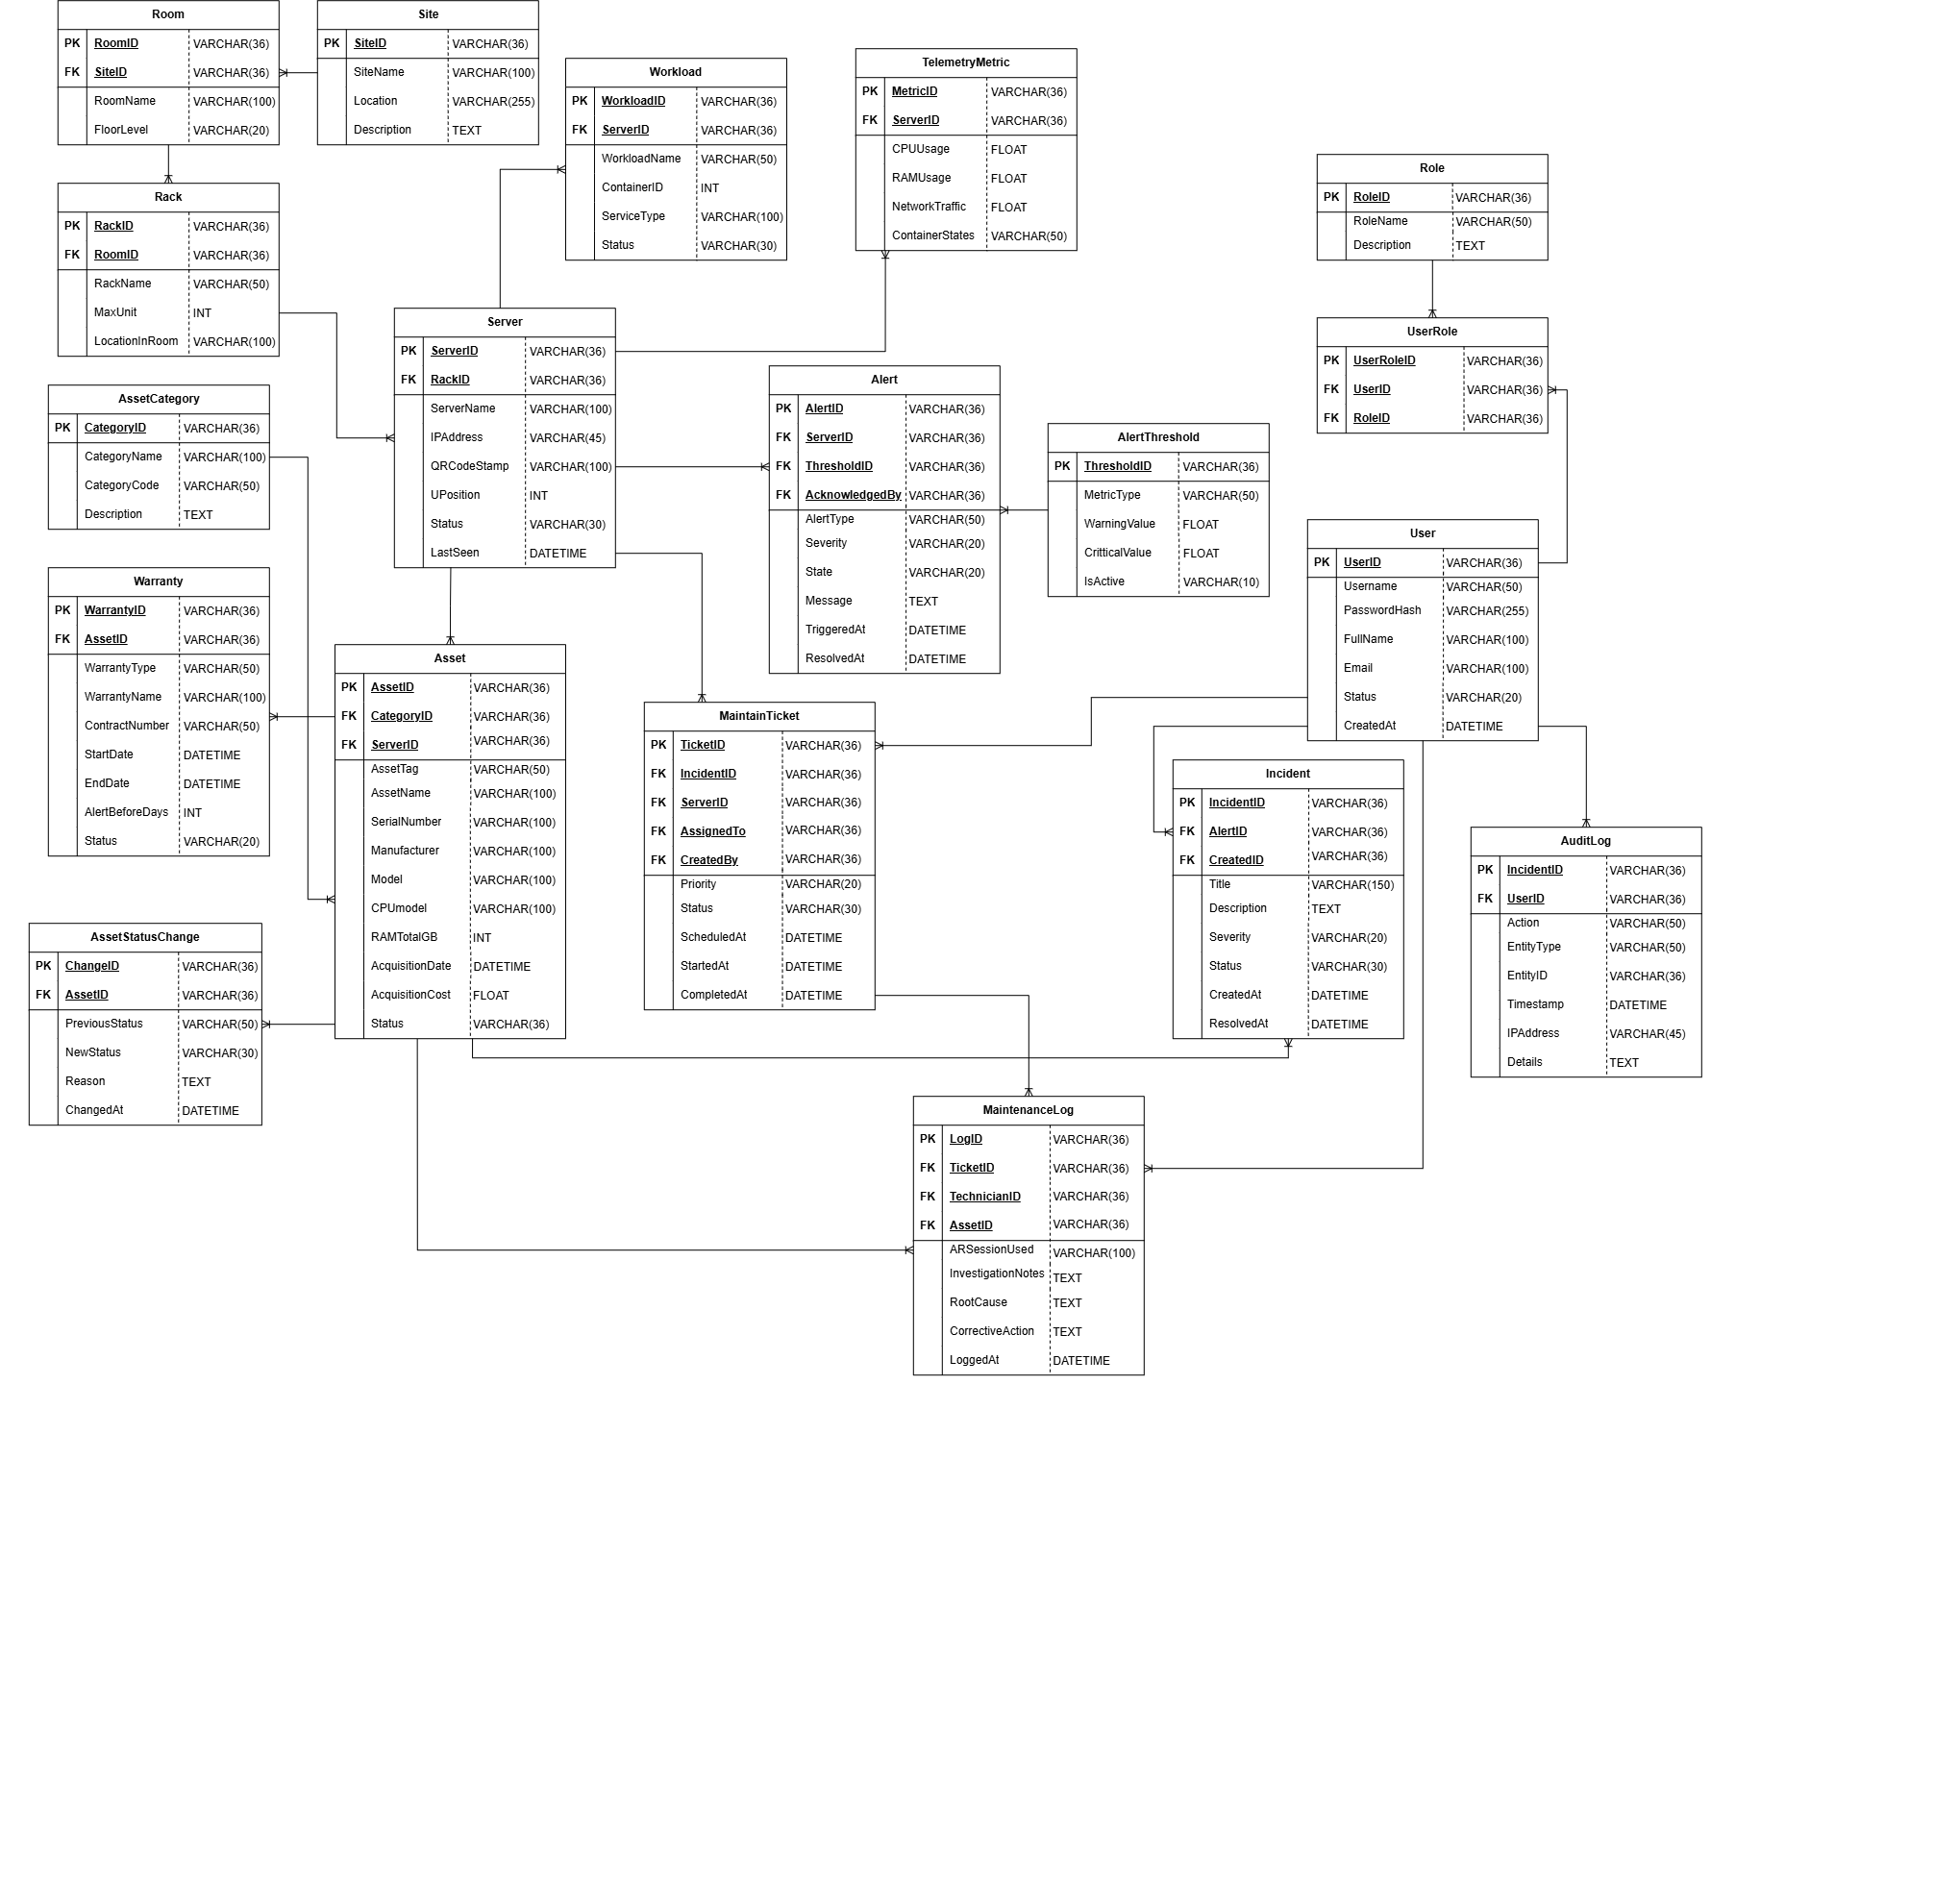
\includegraphics[width=1.0\textwidth]{images/relational_schema.png} 
    \caption{Lược đồ Quan hệ chi tiết hệ thống Quản lý Mini Data Center}
    \label{fig:relational_schema}
\end{figure}

% Ky Anh
\documentclass[12pt,a4paper]{article}

% --- KHU VỰC PREAMBLE ---
\usepackage[utf8]{vietnam}
\usepackage{amsmath,amssymb}
\usepackage{hyperref}
\usepackage{geometry}
\geometry{a4paper, margin=2cm}
\usepackage{float}
\usepackage{tabularx}

\begin{document}

\section*{3.2 Chi tiết các bảng sau khi chuẩn hóa}

Dựa trên quá trình phân rã và thiết kế mô hình quan hệ cho hệ thống quản lý hạ tầng Mini Data Center (AR-IMMS), toàn bộ hệ thống được tổ chức thành 19 bảng thuộc 4 phân hệ chức năng. Các bảng được chuẩn hóa đạt dạng chuẩn \textbf{BCNF / 3NF} nhằm triệt tiêu dư thừa dữ liệu và đảm bảo tính toàn vẹn tham chiếu.

\subsection*{3.2.1 Phân hệ Hạ tầng \& Không gian Vật lý}

\begin{table}[H]
\centering
\caption{Chi tiết cấu trúc các bảng thuộc Phân hệ Hạ tầng \& Không gian Vật lý}
\label{tab:ph_hatang}
\small
\begin{tabularx}{\textwidth}{|c|l|X|X|c|}
\hline
\textbf{STT} & \textbf{Tên bảng} & \textbf{Cấu trúc thuộc tính (PK / FK)} & \textbf{Mô tả nghiệp vụ} & \textbf{Chuẩn} \\ \hline
1 & \texttt{Site} & \underline{\texttt{SiteID}}, \texttt{SiteName}, \texttt{Location}, \texttt{Description} & Lưu trữ vị trí các trung tâm dữ liệu vật lý. & BCNF \\ \hline
2 & \texttt{Room} & \underline{\texttt{RoomID}}, \texttt{RoomName}, \texttt{Floor}, \texttt{SiteID} (FK) & Quản lý phòng máy chuyên dụng thuộc một Site. & BCNF \\ \hline
3 & \texttt{Rack} & \underline{\texttt{RackID}}, \texttt{RackName}, \texttt{MaxUnit}, \texttt{RoomID} (FK) & Quản lý tủ rack chứa thiết bị trong phòng máy. & BCNF \\ \hline
4 & \texttt{Server} & \underline{\texttt{ServerID}}, \texttt{ServerName}, \texttt{IPAddress}, \texttt{UPosition}, \texttt{Status}, \texttt{QRCodeStamp}, \texttt{RackID} (FK) & Quản lý máy chủ vật lý lắp đặt trong tủ Rack. & BCNF \\ \hline
5 & \texttt{Workload} & \underline{\texttt{WorkloadID}}, \texttt{WorkloadName}, \texttt{Type}, \texttt{Status}, \texttt{ServerID} (FK) & Quản lý các dịch vụ ảo hóa, container trên máy chủ. & BCNF \\ \hline
\end{tabularx}
\end{table}

\subsection*{3.2.2 Phân hệ Giám sát \& Vận hành Hệ thống}

\begin{table}[H]
\centering
\caption{Chi tiết cấu trúc các bảng thuộc Phân hệ Giám sát \& Vận hành}
\label{tab:ph_giamsat}
\small
\begin{tabularx}{\textwidth}{|c|l|X|X|c|}
\hline
\textbf{STT} & \textbf{Tên bảng} & \textbf{Cấu trúc thuộc tính (PK / FK)} & \textbf{Mô tả nghiệp vụ} & \textbf{Chuẩn} \\ \hline
6 & \texttt{TelemetryMetric} & \underline{\texttt{MetricID}}, \texttt{CPUUsage}, \texttt{RAMUsage}, \texttt{NetworkTraffic}, \texttt{RecordedAt}, \texttt{ServerID} (FK) & Ghi nhận chỉ số hiệu năng theo chuỗi thời gian real-time. & BCNF \\ \hline
7 & \texttt{AlertThreshold} & \underline{\texttt{ThresholdID}}, \texttt{MetricType}, \texttt{WarningValue}, \texttt{CriticalValue}, \texttt{IsActive} & Cấu hình các ngưỡng cảnh báo động cho chỉ số. & BCNF \\ \hline
8 & \texttt{Alert} & \underline{\texttt{AlertID}}, \texttt{Severity}, \texttt{State}, \texttt{TriggeredAt}, \texttt{ResolvedAt}, \texttt{ServerID} (FK), \texttt{ThresholdID} (FK), \texttt{AcknowledgedBy} (FK) & Ghi nhận sự kiện cảnh báo phát sinh khi vượt ngưỡng. & BCNF \\ \hline
9 & \texttt{Incident} & \underline{\texttt{IncidentID}}, \texttt{Title}, \texttt{Severity}, \texttt{Status}, \texttt{CreatedAt}, \texttt{ResolvedAt}, \texttt{AlertID} (FK), \texttt{CreatedBy} (FK) & Quản lý sự cố nghiêm trọng cần xử lý cấp thiết. & BCNF \\ \hline
10 & \texttt{MaintainTicket} & \underline{\texttt{TicketID}}, \texttt{Title}, \texttt{Priority}, \texttt{Status}, \texttt{ScheduledAt}, \texttt{StartedAt}, \texttt{CompletedAt}, \texttt{IncidentID} (FK), \texttt{ServerID} (FK), \texttt{AssignedTo} (FK), \texttt{CreatedBy} (FK) & Lập phiếu và theo dõi vòng đời bảo trì thiết bị. & BCNF \\ \hline
11 & \texttt{MaintenanceLog} & \underline{\texttt{LogID}}, \texttt{Note}, \texttt{LoggedAt}, \texttt{ARSessionUsed}, \texttt{TicketID} (FK), \texttt{TechnicianID} (FK), \texttt{AssetID} (FK) & Chi tiết nhật ký xử lý kỹ thuật và thao tác kính AR. & BCNF \\ \hline
\end{tabularx}
\end{table}

\subsection*{3.2.3 Phân hệ Quản lý Tài sản \& Bảo hành}

\begin{table}[H]
\centering
\caption{Chi tiết cấu trúc các bảng thuộc Phân hệ Quản lý Tài sản \& Bảo hành}
\label{tab:ph_taisan}
\small
\begin{tabularx}{\textwidth}{|c|l|X|X|c|}
\hline
\textbf{STT} & \textbf{Tên bảng} & \textbf{Cấu trúc thuộc tính (PK / FK)} & \textbf{Mô tả nghiệp vụ} & \textbf{Chuẩn} \\ \hline
12 & \texttt{AssetCategory} & \underline{\texttt{CategoryID}}, \texttt{CategoryCode}, \texttt{CategoryName} & Danh mục phân loại tài sản phần cứng. & BCNF \\ \hline
13 & \texttt{Asset} & \underline{\texttt{AssetID}}, \texttt{AssetTag}, \texttt{SerialNumber}, \texttt{Status}, \texttt{AcquisitionDate}, \texttt{AcquisitionCost}, \texttt{RAMTotalGB}, \texttt{StorageTotalGB}, \texttt{CategoryID} (FK), \texttt{ServerID} (FK) & Quản lý thông tin chi tiết từng tài sản vật lý. & BCNF \\ \hline
14 & \texttt{Warranty} & \underline{\texttt{WarrantyID}}, \texttt{Provider}, \texttt{StartDate}, \texttt{EndDate}, \texttt{AlertBeforeDays}, \texttt{Status}, \texttt{AssetID} (FK) & Theo dõi thời hạn bảo hành với nhà cung cấp. & BCNF \\ \hline
15 & \texttt{AssetStatusChange} & \underline{\texttt{ChangeID}}, \texttt{OldStatus}, \texttt{NewStatus}, \texttt{ChangedAt}, \texttt{Reason}, \texttt{AssetID} (FK) & Lịch sử biến động trạng thái tài sản theo thời gian. & BCNF \\ \hline
\end{tabularx}
\end{table}

\subsection*{3.2.4 Phân hệ Bảo mật, Phân quyền \& Kiểm toán}

\begin{table}[H]
\centering
\caption{Chi tiết cấu trúc các bảng thuộc Phân hệ Bảo mật, Phân quyền \& Kiểm toán}
\label{tab:ph_baomat}
\small
\begin{tabularx}{\textwidth}{|c|l|X|X|c|}
\hline
\textbf{STT} & \textbf{Tên bảng} & \textbf{Cấu trúc thuộc tính (PK / FK)} & \textbf{Mô tả nghiệp vụ} & \textbf{Chuẩn} \\ \hline
16 & \texttt{User} & \underline{\texttt{UserID}}, \texttt{Username}, \texttt{PasswordHash}, \texttt{FullName}, \texttt{Email}, \texttt{Status} & Quản lý thông tin tài khoản người dùng. & BCNF \\ \hline
17 & \texttt{Role} & \underline{\texttt{RoleID}}, \texttt{RoleName}, \texttt{Description} & Định nghĩa các vai trò chức năng hệ thống. & BCNF \\ \hline
18 & \texttt{UserRole} & \underline{\texttt{UserRoleID}}, \texttt{UserID} (FK), \texttt{RoleID} (FK) & Bảng trung gian phân quyền nhiều - nhiều ($N-M$). & BCNF \\ \hline
19 & \texttt{AuditLog} & \underline{\texttt{LogID}}, \texttt{Action}, \texttt{EntityName}, \texttt{EntityID}, \texttt{IPAddress}, \texttt{Timestamp}, \texttt{UserID} (FK) & Lưu nhật ký kiểm toán và truy vết thao tác. & BCNF \\ \hline
\end{tabularx}
\end{table}

\subsection*{3.2.5 Đánh giá Dạng chuẩn toàn hệ thống}
Tất cả 19 bảng đều đạt dạng chuẩn \textbf{BCNF} (Boyce-Codd Normal Form) do thỏa mãn:
\begin{enumerate}
    \item Đạt chuẩn 1NF, 2NF và 3NF (không tồn tại phụ thuộc hàm một phần hay bắc cầu).
    \item Mọi vế trái $X$ của phụ thuộc hàm không tầm thường $X \rightarrow Y$ trong các bảng đều là siêu khóa (Superkey).
    \item Quá trình phân rã bảo toàn hoàn toàn tập phụ thuộc hàm và không làm mất thông tin (Lossless Join).
\end{enumerate}

\end{document}

%hieu
%hieu
\subsection{Ràng buộc Toàn vẹn Dữ liệu}

Phần này trình bày chi tiết các ràng buộc toàn vẹn (Integrity Constraints) được áp dụng trên toàn bộ lược đồ cơ sở dữ liệu của hệ thống AR-IMMS, nhằm đảm bảo tính nhất quán, chính xác và hợp lệ của dữ liệu trong suốt vòng đời vận hành. Các ràng buộc được phân loại thành 5 nhóm chính.

%% =============================================
%% 3.3.1 RÀNG BUỘC KHÓA CHÍNH
%% =============================================
\subsubsection{Ràng buộc Khóa chính (Primary Key Constraints)}

Mỗi bảng trong lược đồ đều được xác định một khóa chính duy nhất, đảm bảo mỗi bản ghi có thể được phân biệt một cách chính xác. Tất cả khóa chính đều có ràng buộc \texttt{NOT NULL} và \texttt{UNIQUE} ngầm định.

\begin{table}[H]
\centering
\caption{Tổng hợp ràng buộc khóa chính của các bảng}
\label{tab:pk_constraints}
\begin{tabular}{|c|l|l|p{5.5cm}|}
\hline
\textbf{STT} & \textbf{Bảng} & \textbf{Khóa chính} & \textbf{Ghi chú} \\ \hline
1 & Site & SiteID & Định danh trung tâm dữ liệu \\ \hline
2 & Room & RoomID & Định danh phòng máy \\ \hline
3 & Rack & RackID & Định danh tủ Rack \\ \hline
4 & Server & ServerID & Nút gốc trung tâm hạ tầng \\ \hline
5 & Workload & WorkloadID & Định danh khối tải công việc \\ \hline
6 & TelemetryMetric & MetricID & Định danh bản ghi đo lường \\ \hline
7 & AlertThreshold & ThresholdID & Định danh cấu hình ngưỡng \\ \hline
8 & Alert & AlertID & Định danh sự kiện cảnh báo \\ \hline
9 & Incident & IncidentID & Định danh sự cố \\ \hline
10 & MaintenanceTicket & TicketID & Định danh phiếu bảo trì \\ \hline
11 & MaintenanceLog & LogID & Định danh nhật ký xử lý \\ \hline
12 & AssetCategory & CategoryID & Định danh danh mục tài sản \\ \hline
13 & Asset & AssetID & Định danh tài sản phần cứng \\ \hline
14 & Warranty & WarrantyID & Định danh hợp đồng bảo hành \\ \hline
15 & AssetStatusChange & ChangeID & Định danh bản ghi thay đổi \\ \hline
16 & User & UserID & Định danh tài khoản người dùng \\ \hline
17 & Role & RoleID & Định danh vai trò hệ thống \\ \hline
18 & UserRole & UserRoleID & Định danh phân quyền \\ \hline
19 & AuditLog & LogID & Định danh nhật ký kiểm toán \\ \hline
\end{tabular}
\end{table}

%% =============================================
%% 3.3.2 RÀNG BUỘC KHÓA NGOẠI
%% =============================================
\subsubsection{Ràng buộc Khóa ngoại và Tham chiếu (Foreign Key \& Referential Integrity)}

Các ràng buộc khóa ngoại đảm bảo tính toàn vẹn tham chiếu giữa các bảng, tuân theo mô hình phân cấp hạ tầng và các trục liên kết trung tâm đã thiết kế trong Chương 2. Hành vi xử lý khi xóa/cập nhật bản ghi cha được quy định cụ thể theo ngữ cảnh nghiệp vụ.

\begin{longtable}{|c|l|l|l|l|}
\caption{Tổng hợp ràng buộc khóa ngoại và hành vi tham chiếu} \label{tab:fk_constraints} \\
\hline
\textbf{STT} & \textbf{Bảng con} & \textbf{Cột FK} & \textbf{Bảng cha (PK)} & \textbf{ON DELETE} \\ \hline
\endfirsthead
\hline
\textbf{STT} & \textbf{Bảng con} & \textbf{Cột FK} & \textbf{Bảng cha (PK)} & \textbf{ON DELETE} \\ \hline
\endhead
\hline
\endfoot
1 & Room & SiteID & Site(SiteID) & RESTRICT \\ \hline
2 & Rack & RoomID & Room(RoomID) & RESTRICT \\ \hline
3 & Server & RackID & Rack(RackID) & RESTRICT \\ \hline
4 & Workload & ServerID & Server(ServerID) & CASCADE \\ \hline
5 & TelemetryMetric & ServerID & Server(ServerID) & CASCADE \\ \hline
6 & Alert & ServerID & Server(ServerID) & RESTRICT \\ \hline
7 & Alert & ThresholdID & AlertThreshold(ThresholdID) & RESTRICT \\ \hline
8 & Alert & AcknowledgedBy & User(UserID) & SET NULL \\ \hline
9 & Incident & AlertID & Alert(AlertID) & SET NULL \\ \hline
10 & Incident & CreatedBy & User(UserID) & RESTRICT \\ \hline
11 & MaintenanceTicket & IncidentID & Incident(IncidentID) & SET NULL \\ \hline
12 & MaintenanceTicket & ServerID & Server(ServerID) & RESTRICT \\ \hline
13 & MaintenanceTicket & AssignedTo & User(UserID) & SET NULL \\ \hline
14 & MaintenanceTicket & CreatedBy & User(UserID) & RESTRICT \\ \hline
15 & MaintenanceLog & TicketID & MaintenanceTicket(TicketID) & CASCADE \\ \hline
16 & MaintenanceLog & TechnicianID & User(UserID) & RESTRICT \\ \hline
17 & MaintenanceLog & AssetID & Asset(AssetID) & SET NULL \\ \hline
18 & Asset & CategoryID & AssetCategory(CategoryID) & RESTRICT \\ \hline
19 & Asset & ServerID & Server(ServerID) & SET NULL \\ \hline
20 & Warranty & AssetID & Asset(AssetID) & CASCADE \\ \hline
21 & AssetStatusChange & AssetID & Asset(AssetID) & CASCADE \\ \hline
22 & UserRole & UserID & User(UserID) & CASCADE \\ \hline
23 & UserRole & RoleID & Role(RoleID) & RESTRICT \\ \hline
24 & AuditLog & UserID & User(UserID) & SET NULL \\ \hline
\end{longtable}

\noindent \textbf{Giải thích hành vi ON DELETE:}
\begin{itemize}[leftmargin=2em]
    \item \texttt{RESTRICT}: Không cho phép xóa bản ghi cha khi còn tồn tại bản ghi con tham chiếu. Áp dụng cho các thực thể phân cấp hạ tầng (Site $\rightarrow$ Room $\rightarrow$ Rack $\rightarrow$ Server) nhằm tránh mất dữ liệu cấu hình quan trọng (theo quy tắc BR-1).
    \item \texttt{CASCADE}: Xóa tự động các bản ghi con khi bản ghi cha bị xóa. Áp dụng cho dữ liệu phụ thuộc hoàn toàn (Workload, TelemetryMetric, MaintenanceLog, Warranty, AssetStatusChange, UserRole).
    \item \texttt{SET NULL}: Đặt giá trị cột FK thành \texttt{NULL} khi bản ghi cha bị xóa. Áp dụng cho các trường tham chiếu tùy chọn (AcknowledgedBy, AssignedTo, AlertID trong Incident).
\end{itemize}

%% =============================================
%% 3.3.3 RÀNG BUỘC MIỀN GIÁ TRỊ
%% =============================================
\subsubsection{Ràng buộc Miền giá trị (Domain \& CHECK Constraints)}

Các ràng buộc miền giá trị giới hạn tập giá trị hợp lệ cho từng thuộc tính, bao gồm ràng buộc \texttt{CHECK} cho giá trị số và ràng buộc kiểu liệt kê (\texttt{ENUM} / \texttt{CHECK IN}) cho các trường trạng thái.

\vspace{0.5em}
\noindent\textbf{a) Ràng buộc giá trị số (Numeric CHECK):}

\begin{longtable}{|l|l|p{6cm}|}
\caption{Ràng buộc CHECK cho các thuộc tính số} \label{tab:check_numeric} \\
\hline
\textbf{Bảng} & \textbf{Thuộc tính} & \textbf{Biểu thức ràng buộc} \\ \hline
\endfirsthead
\hline
\textbf{Bảng} & \textbf{Thuộc tính} & \textbf{Biểu thức ràng buộc} \\ \hline
\endhead
\hline
\endfoot
Rack & MaxUnit & \texttt{MaxUnit > 0} \\ \hline
Server & UPosition & \texttt{UPosition > 0} \\ \hline
TelemetryMetric & CPUUsage & \texttt{CPUUsage >= 0 AND CPUUsage <= 100} \\ \hline
TelemetryMetric & RAMUsage & \texttt{RAMUsage >= 0 AND RAMUsage <= 100} \\ \hline
TelemetryMetric & NetworkTraffic & \texttt{NetworkTraffic >= 0} \\ \hline
AlertThreshold & WarningValue & \texttt{WarningValue > 0} \\ \hline
AlertThreshold & CriticalValue & \texttt{CriticalValue > WarningValue} \\ \hline
Asset & RAMTotalGB & \texttt{RAMTotalGB > 0} \\ \hline
Asset & StorageTotalGB & \texttt{StorageTotalGB > 0} \\ \hline
Asset & AcquisitionCost & \texttt{AcquisitionCost >= 0} \\ \hline
Warranty & AlertBeforeDays & \texttt{AlertBeforeDays > 0} \\ \hline
\end{longtable}

\vspace{0.5em}
\noindent\textbf{b) Ràng buộc kiểu liệt kê trạng thái (ENUM / CHECK IN):}

Các trường trạng thái được ràng buộc theo tập giá trị hữu hạn, đảm bảo máy trạng thái (state machine) chỉ chấp nhận các giá trị hợp lệ đã quy định trong quy tắc nghiệp vụ.

\begin{longtable}{|l|l|p{7.5cm}|}
\caption{Ràng buộc ENUM cho các trường trạng thái} \label{tab:check_enum} \\
\hline
\textbf{Bảng} & \textbf{Thuộc tính} & \textbf{Tập giá trị hợp lệ} \\ \hline
\endfirsthead
\hline
\textbf{Bảng} & \textbf{Thuộc tính} & \textbf{Tập giá trị hợp lệ} \\ \hline
\endhead
\hline
\endfoot
Server & Status & \texttt{\{'Online', 'Offline', 'Maintenance', 'Critical', 'Unavailable'\}} \\ \hline
Workload & Status & \texttt{\{'Running', 'Stopped', 'Error', 'Deploying'\}} \\ \hline
Alert & Severity & \texttt{\{'Warning', 'Critical'\}} \\ \hline
Alert & State & \texttt{\{'Open', 'Acknowledged', 'Resolved', 'Closed'\}} (theo BR-3) \\ \hline
Incident & Severity & \texttt{\{'Low', 'Medium', 'High', 'Critical'\}} \\ \hline
Incident & Status & \texttt{\{'Open', 'In\_Progress', 'Resolved', 'Closed'\}} \\ \hline
MaintenanceTicket & Priority & \texttt{\{'Low', 'Medium', 'High', 'Urgent'\}} \\ \hline
MaintenanceTicket & Status & \texttt{\{'Assigned', 'In\_Progress', 'Pending\_Approval', 'Closed'\}} (theo BR-4) \\ \hline
Asset & Status & \texttt{\{'Active', 'Spare', 'In\_Repair', 'Decommissioned', 'Disposed'\}} \\ \hline
Warranty & Status & \texttt{\{'Active', 'Expired', 'Claimed'\}} \\ \hline
User & Status & \texttt{\{'Active', 'Inactive', 'Locked'\}} \\ \hline
AlertThreshold & IsActive & \texttt{\{TRUE, FALSE\}} (kiểu BOOLEAN) \\ \hline
\end{longtable}

%% =============================================
%% 3.3.4 RÀNG BUỘC DUY NHẤT
%% =============================================
\subsubsection{Ràng buộc Duy nhất (UNIQUE Constraints)}

Ngoài khóa chính, một số thuộc tính yêu cầu tính duy nhất trên toàn hệ thống để đảm bảo không trùng lặp dữ liệu định danh.

\begin{table}[H]
\centering
\caption{Các ràng buộc UNIQUE trên các bảng}
\label{tab:unique_constraints}
\begin{tabular}{|l|l|p{6.5cm}|}
\hline
\textbf{Bảng} & \textbf{Thuộc tính} & \textbf{Ý nghĩa nghiệp vụ} \\ \hline
User & Username & Tên đăng nhập không được trùng lặp \\ \hline
User & Email & Địa chỉ email duy nhất trên hệ thống \\ \hline
Server & IPAddress & Một máy chủ có địa chỉ IP quản lý duy nhất \\ \hline
Server & QRCodeStamp & Mã QR/ArUco Marker duy nhất (theo BR-2) \\ \hline
Asset & AssetTag & Mã thẻ quản lý tài sản không trùng lặp \\ \hline
Asset & SerialNumber & Số sê-ri phần cứng duy nhất \\ \hline
AssetCategory & CategoryCode & Mã viết tắt danh mục không trùng lặp \\ \hline
UserRole & (UserID, RoleID) & Một người dùng không được gán cùng một vai trò hai lần \\ \hline
\end{tabular}
\end{table}

%% =============================================
%% 3.3.5 RÀNG BUỘC LIÊN THUỘC TÍNH & LOGIC THỜI GIAN
%% =============================================
\subsubsection{Ràng buộc Liên thuộc tính và Logic Thời gian (Inter-attribute \& Temporal Constraints)}

Các ràng buộc sau đảm bảo tính nhất quán logic giữa nhiều thuộc tính trong cùng một bản ghi hoặc giữa các bảng liên quan, đặc biệt là các ràng buộc về trình tự thời gian trong vòng đời xử lý.

\vspace{0.5em}
\noindent\textbf{a) Ràng buộc thứ tự thời gian (Temporal Ordering):}

\begin{longtable}{|l|p{9cm}|}
\caption{Ràng buộc trình tự thời gian giữa các thuộc tính} \label{tab:temporal_constraints} \\
\hline
\textbf{Bảng} & \textbf{Biểu thức ràng buộc} \\ \hline
\endfirsthead
\hline
\textbf{Bảng} & \textbf{Biểu thức ràng buộc} \\ \hline
\endhead
\hline
\endfoot
Alert & \texttt{ResolvedAt IS NULL OR ResolvedAt >= TriggeredAt} \\ \hline
Incident & \texttt{ResolvedAt IS NULL OR ResolvedAt >= CreatedAt} \\ \hline
MaintenanceTicket & \texttt{StartedAt IS NULL OR StartedAt >= ScheduledAt} \\ \hline
MaintenanceTicket & \texttt{CompletedAt IS NULL OR CompletedAt >= StartedAt} \\ \hline
MaintenanceLog & \texttt{LoggedAt >= (SELECT StartedAt FROM MaintenanceTicket WHERE TicketID = MaintenanceLog.TicketID)} \\ \hline
Warranty & \texttt{EndDate > StartDate} \\ \hline
AssetStatusChange & \texttt{ChangedAt >= (SELECT AcquisitionDate FROM Asset WHERE AssetID = AssetStatusChange.AssetID)} \\ \hline
\end{longtable}

\vspace{0.5em}
\noindent\textbf{b) Ràng buộc liên thuộc tính khác (Inter-attribute Logic):}

\begin{itemize}[leftmargin=2em]
    \item \textbf{Alert -- AcknowledgedBy:} Trường \texttt{AcknowledgedBy} chỉ được phép có giá trị khác \texttt{NULL} khi \texttt{Alert.State} đang ở trạng thái \texttt{'Acknowledged'}, \texttt{'Resolved'} hoặc \texttt{'Closed'}.
    \[
    \texttt{State} = \text{'Open'} \implies \texttt{AcknowledgedBy IS NULL}
    \]
    
    \item \textbf{MaintenanceTicket -- AssignedTo:} Khi phiếu bảo trì đang ở trạng thái \texttt{'In\_Progress'}, trường \texttt{AssignedTo} bắt buộc phải có giá trị (không được \texttt{NULL}).
    \[
    \texttt{Status} = \text{'In\_Progress'} \implies \texttt{AssignedTo IS NOT NULL}
    \]
    
    \item \textbf{MaintenanceTicket -- CompletedAt:} Trường \texttt{CompletedAt} chỉ được phép có giá trị khi phiếu ở trạng thái \texttt{'Pending\_Approval'} hoặc \texttt{'Closed'}.
    \[
    \texttt{CompletedAt IS NOT NULL} \implies \texttt{Status} \in \{\text{'Pending\_Approval'},\ \text{'Closed'}\}
    \]
    
    \item \textbf{Incident -- ResolvedAt:} Trường \texttt{ResolvedAt} chỉ có giá trị khi sự cố đã được xử lý.
    \[
    \texttt{ResolvedAt IS NOT NULL} \implies \texttt{Status} \in \{\text{'Resolved'},\ \text{'Closed'}\}
    \]
    
    \item \textbf{Server -- Workload cascade (BR-1, Quy tắc nghiệp vụ):} Khi trạng thái máy chủ chuyển sang \texttt{'Offline'} hoặc \texttt{'Critical'}, tất cả \texttt{Workload} đang chạy trên máy chủ đó phải tự động chuyển trạng thái sang \texttt{'Stopped'}. Ràng buộc này được thực thi thông qua Trigger cơ sở dữ liệu.
\end{itemize}

\vspace{0.5em}
\noindent\textbf{c) Ràng buộc bất biến dữ liệu (Immutability):}

\begin{itemize}[leftmargin=2em]
    \item \textbf{AuditLog (BR-10):} Bảng \texttt{AuditLog} chỉ cho phép thao tác \texttt{INSERT}. Mọi thao tác \texttt{UPDATE} hoặc \texttt{DELETE} trên bảng này đều bị từ chối bởi Trigger bảo vệ.
    \item \textbf{TelemetryMetric:} Các bản ghi telemetry sau khi được ghi nhận không được phép chỉnh sửa (\texttt{UPDATE}) nhằm đảm bảo tính trung thực của dữ liệu chuỗi thời gian.
\end{itemize}

\vspace{0.5em}
\noindent\textbf{d) Ràng buộc máy trạng thái -- chuyển trạng thái hợp lệ (State Machine Constraints):}

Dựa trên các quy tắc nghiệp vụ BR-3 và BR-4, các chuyển đổi trạng thái chỉ được phép theo chiều thuận, không cho phép quay ngược. Các ràng buộc này được thực thi thông qua Trigger \texttt{BEFORE UPDATE}.

\begin{itemize}[leftmargin=2em]
    \item \textbf{Alert.State (BR-3):} Chỉ cho phép các chuyển trạng thái hợp lệ:
    \[
    \texttt{Open} \rightarrow \texttt{Acknowledged} \rightarrow \texttt{Resolved} \rightarrow \texttt{Closed}
    \]
    
    \item \textbf{MaintenanceTicket.Status (BR-4):} Chỉ cho phép:
    \[
    \texttt{Assigned} \rightarrow \texttt{In\_Progress} \rightarrow \texttt{Pending\_Approval} \rightarrow \texttt{Closed}
    \]
    
    \item \textbf{Incident.Status:} Chỉ cho phép:
    \[
    \texttt{Open} \rightarrow \texttt{In\_Progress} \rightarrow \texttt{Resolved} \rightarrow \texttt{Closed}
    \]
\end{itemize}

\vspace{0.5em}
\noindent\textbf{e) Ràng buộc phân quyền nghiệp vụ (RBAC Business Constraints):}

\begin{itemize}[leftmargin=2em]
    \item \textbf{Xác nhận cảnh báo (BR-5):} Chỉ \texttt{User} có \texttt{Role} là \textit{``Operator''} hoặc \textit{``System Admin''} mới được phép cập nhật trường \texttt{Alert.AcknowledgedBy} và chuyển trạng thái \texttt{Alert.State} sang \texttt{'Acknowledged'}.
    \item \textbf{Phê duyệt đóng phiếu (BR-5):} Chỉ \texttt{User} có \texttt{Role} là \textit{``Operator''} mới được phép chuyển trạng thái \texttt{MaintenanceTicket.Status} từ \texttt{'Pending\_Approval'} sang \texttt{'Closed'}. Kỹ thuật viên (\textit{Technician}) chỉ được phép chuyển sang \texttt{'Pending\_Approval'}.
\end{itemize}



\chapter{Thiết kế Vật lý \& Code Script SQL}
\clearpage

\chapter{Thiết kế vật lý Cơ sở dữ liệu}

% Hieu
\section{Hiện thực cấu trúc bảng}

Phần này trình bày toàn bộ mã lệnh SQL hiện thực hóa cấu trúc vật lý của 19 bảng trong cơ sở dữ liệu \texttt{DataCenterManagement\_DB} trên hệ quản trị \textbf{Microsoft SQL Server}. Các bảng được tổ chức theo 4 phân hệ chức năng đã thiết kế tại Chương 3, bao gồm: định nghĩa kiểu dữ liệu, khóa chính (\texttt{PRIMARY KEY}), khóa ngoại (\texttt{FOREIGN KEY REFERENCES}), và ràng buộc \texttt{NOT NULL}.

\vspace{0.5em}
\noindent Trước tiên, tạo cơ sở dữ liệu và chuyển ngữ cảnh sử dụng:

\begin{tcolorbox}[colback=gray!5, colframe=gray!60, title={\textbf{Khởi tạo Database}}, fonttitle=\bfseries\small, boxrule=0.5pt, arc=2pt]
\begin{lstlisting}[language=SQL, basicstyle=\ttfamily\small, breaklines=true, showstringspaces=false, keywordstyle=\bfseries\color{blue!70!black}, stringstyle=\color{red!70!black}, commentstyle=\itshape\color{green!50!black}]
CREATE DATABASE DataCenterManagement_DB;
GO

USE DataCenterManagement_DB;
GO
\end{lstlisting}
\end{tcolorbox}

%% =============================================
%% 4.1.1 PHAN HE HA TANG & KHONG GIAN VAT LY
%% =============================================
\subsection{Phân hệ Hạ tầng \& Không gian Vật lý}

Phân hệ này gồm 5 bảng mô tả cấu trúc phân cấp vật lý của trung tâm dữ liệu: \texttt{Site} $\rightarrow$ \texttt{Room} $\rightarrow$ \texttt{Rack} $\rightarrow$ \texttt{Server} $\rightarrow$ \texttt{Workload}. Mỗi bảng con tham chiếu khóa ngoại đến bảng cha, thể hiện quan hệ chứa -- thuộc.

\vspace{0.5em}
\noindent\textbf{Bảng Site} -- Lưu trữ thông tin các trung tâm dữ liệu vật lý (Data Center Site).

\begin{tcolorbox}[colback=gray!5, colframe=gray!60, title={\textbf{CREATE TABLE Site}}, fonttitle=\bfseries\small, boxrule=0.5pt, arc=2pt]
\begin{lstlisting}[language=SQL, basicstyle=\ttfamily\small, breaklines=true, showstringspaces=false, keywordstyle=\bfseries\color{blue!70!black}, stringstyle=\color{red!70!black}, commentstyle=\itshape\color{green!50!black}]
CREATE TABLE Site (
    SiteID       VARCHAR(36) PRIMARY KEY,
    SiteName     VARCHAR(50) NOT NULL,
    Location     VARCHAR(255),
    Description  TEXT
);
\end{lstlisting}
\end{tcolorbox}

\begin{itemize}[leftmargin=2em]
    \item \texttt{SiteID}: Khóa chính, định danh duy nhất cho mỗi trung tâm dữ liệu.
    \item \texttt{SiteName}: Tên trung tâm dữ liệu, bắt buộc nhập (\texttt{NOT NULL}).
    \item \texttt{Location}: Địa chỉ vị trí địa lý, cho phép \texttt{NULL}.
    \item \texttt{Description}: Mô tả chi tiết bổ sung, kiểu \texttt{TEXT}.
\end{itemize}

\vspace{0.5em}
\noindent\textbf{Bảng Room} -- Quản lý các phòng máy chuyên dụng thuộc một Site.

\begin{tcolorbox}[colback=gray!5, colframe=gray!60, title={\textbf{CREATE TABLE Room}}, fonttitle=\bfseries\small, boxrule=0.5pt, arc=2pt]
\begin{lstlisting}[language=SQL, basicstyle=\ttfamily\small, breaklines=true, showstringspaces=false, keywordstyle=\bfseries\color{blue!70!black}, stringstyle=\color{red!70!black}, commentstyle=\itshape\color{green!50!black}]
CREATE TABLE Room (
    RoomID     VARCHAR(36) PRIMARY KEY,
    SiteID     VARCHAR(36) FOREIGN KEY REFERENCES Site(SiteID),
    RoomName   VARCHAR(30) NOT NULL,
    FloorLevel VARCHAR(10)
);
\end{lstlisting}
\end{tcolorbox}

\begin{itemize}[leftmargin=2em]
    \item \texttt{RoomID}: Khóa chính, định danh phòng máy.
    \item \texttt{SiteID}: Khóa ngoại tham chiếu đến \texttt{Site(SiteID)}, xác định phòng thuộc trung tâm dữ liệu nào.
    \item \texttt{RoomName}: Tên phòng máy, bắt buộc nhập.
    \item \texttt{FloorLevel}: Tầng đặt phòng máy.
\end{itemize}

\vspace{0.5em}
\noindent\textbf{Bảng Rack} -- Quản lý các tủ rack chứa thiết bị trong phòng máy.

\begin{tcolorbox}[colback=gray!5, colframe=gray!60, title={\textbf{CREATE TABLE Rack}}, fonttitle=\bfseries\small, boxrule=0.5pt, arc=2pt]
\begin{lstlisting}[language=SQL, basicstyle=\ttfamily\small, breaklines=true, showstringspaces=false, keywordstyle=\bfseries\color{blue!70!black}, stringstyle=\color{red!70!black}, commentstyle=\itshape\color{green!50!black}]
CREATE TABLE Rack (
    RackID         VARCHAR(36) PRIMARY KEY,
    RoomID         VARCHAR(36) FOREIGN KEY REFERENCES Room(RoomID),
    RackName       VARCHAR(30) NOT NULL,
    MaxUnit        INT,
    LocationInRoom VARCHAR(50)
);
\end{lstlisting}
\end{tcolorbox}

\begin{itemize}[leftmargin=2em]
    \item \texttt{RackID}: Khóa chính, định danh tủ rack.
    \item \texttt{RoomID}: Khóa ngoại tham chiếu đến \texttt{Room(RoomID)}.
    \item \texttt{RackName}: Tên tủ rack, bắt buộc nhập.
    \item \texttt{MaxUnit}: Số đơn vị U tối đa mà rack hỗ trợ (kiểu \texttt{INT}).
    \item \texttt{LocationInRoom}: Vị trí đặt rack trong phòng máy.
\end{itemize}

\vspace{0.5em}
\noindent\textbf{Bảng Server} -- Quản lý máy chủ vật lý lắp đặt trong tủ Rack.

\begin{tcolorbox}[colback=gray!5, colframe=gray!60, title={\textbf{CREATE TABLE Server}}, fonttitle=\bfseries\small, boxrule=0.5pt, arc=2pt]
\begin{lstlisting}[language=SQL, basicstyle=\ttfamily\small, breaklines=true, showstringspaces=false, keywordstyle=\bfseries\color{blue!70!black}, stringstyle=\color{red!70!black}, commentstyle=\itshape\color{green!50!black}]
CREATE TABLE Server (
    ServerID    VARCHAR(36) PRIMARY KEY,
    RackID      VARCHAR(36) FOREIGN KEY REFERENCES Rack(RackID),
    ServerName  VARCHAR(40) NOT NULL,
    IPAddress   VARCHAR(45),
    QRCodeStamp VARCHAR(50),
    UPosition   INT,
    Status      VARCHAR(20),
    LastSeen    DATETIME
);
\end{lstlisting}
\end{tcolorbox}

\begin{itemize}[leftmargin=2em]
    \item \texttt{ServerID}: Khóa chính, định danh máy chủ.
    \item \texttt{RackID}: Khóa ngoại tham chiếu đến \texttt{Rack(RackID)}.
    \item \texttt{ServerName}: Tên máy chủ, bắt buộc nhập.
    \item \texttt{IPAddress}: Địa chỉ IP quản lý, hỗ trợ cả IPv4/IPv6 (\texttt{VARCHAR(45)}).
    \item \texttt{QRCodeStamp}: Mã QR/ArUco Marker dán trên thiết bị vật lý, phục vụ nhận diện AR.
    \item \texttt{UPosition}: Vị trí đơn vị U trong rack (kiểu \texttt{INT}).
    \item \texttt{Status}: Trạng thái hoạt động hiện tại của máy chủ.
    \item \texttt{LastSeen}: Thời điểm hệ thống ghi nhận máy chủ trực tuyến lần cuối.
\end{itemize}

\vspace{0.5em}
\noindent\textbf{Bảng Workload} -- Quản lý các dịch vụ ảo hóa, container chạy trên máy chủ.

\begin{tcolorbox}[colback=gray!5, colframe=gray!60, title={\textbf{CREATE TABLE Workload}}, fonttitle=\bfseries\small, boxrule=0.5pt, arc=2pt]
\begin{lstlisting}[language=SQL, basicstyle=\ttfamily\small, breaklines=true, showstringspaces=false, keywordstyle=\bfseries\color{blue!70!black}, stringstyle=\color{red!70!black}, commentstyle=\itshape\color{green!50!black}]
CREATE TABLE Workload (
    WorkloadID   VARCHAR(36) PRIMARY KEY,
    ServerID     VARCHAR(36) FOREIGN KEY REFERENCES Server(ServerID),
    WorkloadName VARCHAR(50) NOT NULL,
    ContainerID  INT,
    ServiceType  VARCHAR(40),
    Status       VARCHAR(20)
);
\end{lstlisting}
\end{tcolorbox}

\begin{itemize}[leftmargin=2em]
    \item \texttt{WorkloadID}: Khóa chính, định danh khối tải công việc.
    \item \texttt{ServerID}: Khóa ngoại tham chiếu đến \texttt{Server(ServerID)}.
    \item \texttt{WorkloadName}: Tên dịch vụ/container, bắt buộc nhập.
    \item \texttt{ContainerID}: Mã định danh container nội bộ (kiểu \texttt{INT}).
    \item \texttt{ServiceType}: Loại dịch vụ (Web Proxy, Database, Microservice, Cache...).
    \item \texttt{Status}: Trạng thái hoạt động của workload.
\end{itemize}

%% =============================================
%% 4.1.2 PHAN HE GIAM SAT & VAN HANH
%% =============================================
\subsection{Phân hệ Giám sát \& Vận hành Hệ thống}

Phân hệ này gồm 6 bảng phục vụ giám sát hiệu năng, quản lý cảnh báo, xử lý sự cố và bảo trì thiết bị: \texttt{TelemetryMetric}, \texttt{AlertThreshold}, \texttt{Alert}, \texttt{Incident}, \texttt{MaintainTicket}, \texttt{MaintenanceLog}.

\vspace{0.5em}
\noindent\textbf{Bảng TelemetryMetric} -- Ghi nhận chỉ số hiệu năng hệ thống theo thời gian thực.

\begin{tcolorbox}[colback=gray!5, colframe=gray!60, title={\textbf{CREATE TABLE TelemetryMetric}}, fonttitle=\bfseries\small, boxrule=0.5pt, arc=2pt]
\begin{lstlisting}[language=SQL, basicstyle=\ttfamily\small, breaklines=true, showstringspaces=false, keywordstyle=\bfseries\color{blue!70!black}, stringstyle=\color{red!70!black}, commentstyle=\itshape\color{green!50!black}]
CREATE TABLE TelemetryMetric (
    MetricID        VARCHAR(36) PRIMARY KEY,
    ServerID        VARCHAR(36) FOREIGN KEY REFERENCES Server(ServerID),
    CPUUsage        FLOAT,
    RAMUsage        FLOAT,
    NetworkTraffic  FLOAT,
    ContainerStates VARCHAR(50)
);
\end{lstlisting}
\end{tcolorbox}

\begin{itemize}[leftmargin=2em]
    \item \texttt{MetricID}: Khóa chính, định danh bản ghi đo lường.
    \item \texttt{ServerID}: Khóa ngoại tham chiếu đến \texttt{Server(ServerID)}, xác định máy chủ được giám sát.
    \item \texttt{CPUUsage}, \texttt{RAMUsage}: Tỷ lệ sử dụng CPU và RAM (kiểu \texttt{FLOAT}, đơn vị \%).
    \item \texttt{NetworkTraffic}: Lưu lượng mạng (kiểu \texttt{FLOAT}, đơn vị Mbps).
    \item \texttt{ContainerStates}: Trạng thái tổng hợp của các container trên máy chủ.
\end{itemize}

\vspace{0.5em}
\noindent\textbf{Bảng AlertThreshold} -- Cấu hình các ngưỡng cảnh báo động cho các chỉ số hiệu năng.

\begin{tcolorbox}[colback=gray!5, colframe=gray!60, title={\textbf{CREATE TABLE AlertThreshold}}, fonttitle=\bfseries\small, boxrule=0.5pt, arc=2pt]
\begin{lstlisting}[language=SQL, basicstyle=\ttfamily\small, breaklines=true, showstringspaces=false, keywordstyle=\bfseries\color{blue!70!black}, stringstyle=\color{red!70!black}, commentstyle=\itshape\color{green!50!black}]
CREATE TABLE AlertThreshold (
    ThresholdID   VARCHAR(36) PRIMARY KEY,
    MetricType    VARCHAR(50),
    WarningValue  FLOAT,
    CriticalValue FLOAT,
    IsActive      BIT
);
\end{lstlisting}
\end{tcolorbox}

\begin{itemize}[leftmargin=2em]
    \item \texttt{ThresholdID}: Khóa chính, định danh cấu hình ngưỡng.
    \item \texttt{MetricType}: Loại chỉ số áp dụng ngưỡng (CPU, RAM, Network).
    \item \texttt{WarningValue}: Giá trị ngưỡng cảnh báo mức Warning (kiểu \texttt{FLOAT}).
    \item \texttt{CriticalValue}: Giá trị ngưỡng cảnh báo mức Critical (kiểu \texttt{FLOAT}).
    \item \texttt{IsActive}: Cờ kích hoạt ngưỡng (kiểu \texttt{BIT}: 0 = tắt, 1 = bật).
\end{itemize}

\vspace{0.5em}
\noindent\textbf{Bảng Alert} -- Ghi nhận các sự kiện cảnh báo phát sinh khi chỉ số vượt ngưỡng.

\begin{tcolorbox}[colback=gray!5, colframe=gray!60, title={\textbf{CREATE TABLE Alert}}, fonttitle=\bfseries\small, boxrule=0.5pt, arc=2pt]
\begin{lstlisting}[language=SQL, basicstyle=\ttfamily\small, breaklines=true, showstringspaces=false, keywordstyle=\bfseries\color{blue!70!black}, stringstyle=\color{red!70!black}, commentstyle=\itshape\color{green!50!black}]
CREATE TABLE Alert (
    AlertID        VARCHAR(36) PRIMARY KEY,
    ServerID       VARCHAR(36) FOREIGN KEY REFERENCES Server(ServerID),
    ThresholdID    VARCHAR(36) FOREIGN KEY REFERENCES
                       AlertThreshold(ThresholdID),
    AcknowledgedBy VARCHAR(36) FOREIGN KEY REFERENCES [User](UserID),
    Alerttype      VARCHAR(30),
    Severity       VARCHAR(15),
    State          VARCHAR(15),
    Message        TEXT,
    TriggeredAt    DATETIME,
    ResolvedAt     DATETIME
);
\end{lstlisting}
\end{tcolorbox}

\begin{itemize}[leftmargin=2em]
    \item \texttt{AlertID}: Khóa chính, định danh sự kiện cảnh báo.
    \item \texttt{ServerID}: Khóa ngoại -- máy chủ phát sinh cảnh báo.
    \item \texttt{ThresholdID}: Khóa ngoại -- cấu hình ngưỡng đã kích hoạt cảnh báo.
    \item \texttt{AcknowledgedBy}: Khóa ngoại -- người dùng xác nhận cảnh báo (cho phép \texttt{NULL} khi chưa xác nhận).
    \item \texttt{Alerttype}: Loại cảnh báo (CPU Spike, RAM High, Network Peak...).
    \item \texttt{Severity}: Mức độ nghiêm trọng (\texttt{Warning}, \texttt{Critical}).
    \item \texttt{State}: Trạng thái vòng đời cảnh báo (\texttt{Open} $\rightarrow$ \texttt{Acknowledged} $\rightarrow$ \texttt{Resolved} $\rightarrow$ \texttt{Closed}).
    \item \texttt{Message}: Nội dung chi tiết thông điệp cảnh báo.
    \item \texttt{TriggeredAt}, \texttt{ResolvedAt}: Thời điểm phát sinh và xử lý xong cảnh báo.
\end{itemize}

\vspace{0.5em}
\noindent\textbf{Bảng Incident} -- Quản lý các sự cố nghiêm trọng cần xử lý cấp thiết.

\begin{tcolorbox}[colback=gray!5, colframe=gray!60, title={\textbf{CREATE TABLE Incident}}, fonttitle=\bfseries\small, boxrule=0.5pt, arc=2pt]
\begin{lstlisting}[language=SQL, basicstyle=\ttfamily\small, breaklines=true, showstringspaces=false, keywordstyle=\bfseries\color{blue!70!black}, stringstyle=\color{red!70!black}, commentstyle=\itshape\color{green!50!black}]
CREATE TABLE Incident (
    IncidentID  VARCHAR(36) PRIMARY KEY,
    CreatedID   VARCHAR(36) FOREIGN KEY REFERENCES [User](UserID),
    Title       VARCHAR(100) NOT NULL,
    Description TEXT,
    Severity    VARCHAR(20),
    Status      VARCHAR(20),
    CreatedAt   DATETIME,
    ResolvedAt  DATETIME
);
\end{lstlisting}
\end{tcolorbox}

\begin{itemize}[leftmargin=2em]
    \item \texttt{IncidentID}: Khóa chính, định danh sự cố.
    \item \texttt{CreatedID}: Khóa ngoại tham chiếu đến \texttt{User(UserID)} -- người tạo báo cáo sự cố.
    \item \texttt{Title}: Tiêu đề mô tả ngắn gọn sự cố, bắt buộc nhập.
    \item \texttt{Description}: Mô tả chi tiết sự cố (kiểu \texttt{TEXT}).
    \item \texttt{Severity}: Mức độ nghiêm trọng (\texttt{Low}, \texttt{Medium}, \texttt{High}, \texttt{Critical}).
    \item \texttt{Status}: Trạng thái xử lý sự cố (\texttt{Open}, \texttt{In Progress}, \texttt{Resolved}, \texttt{Closed}).
    \item \texttt{CreatedAt}, \texttt{ResolvedAt}: Thời điểm tạo và xử lý xong sự cố.
\end{itemize}

\vspace{0.5em}
\noindent\textbf{Bảng MaintainTicket} -- Lập phiếu và theo dõi vòng đời bảo trì thiết bị.

\begin{tcolorbox}[colback=gray!5, colframe=gray!60, title={\textbf{CREATE TABLE MaintainTicket}}, fonttitle=\bfseries\small, boxrule=0.5pt, arc=2pt]
\begin{lstlisting}[language=SQL, basicstyle=\ttfamily\small, breaklines=true, showstringspaces=false, keywordstyle=\bfseries\color{blue!70!black}, stringstyle=\color{red!70!black}, commentstyle=\itshape\color{green!50!black}]
CREATE TABLE MaintainTicket (
    TicketID    VARCHAR(36) PRIMARY KEY,
    IncidentID  VARCHAR(36) FOREIGN KEY REFERENCES
                    Incident(IncidentID),
    ServerID    VARCHAR(36) FOREIGN KEY REFERENCES
                    Server(ServerID),
    AssignedTo  VARCHAR(36) FOREIGN KEY REFERENCES
                    [User](UserID),
    CreatedBy   VARCHAR(36) FOREIGN KEY REFERENCES
                    [User](UserID),
    Priority    VARCHAR(20),
    Status      VARCHAR(20),
    ScheduledAt DATETIME,
    StartedAt   DATETIME,
    CompletedAt DATETIME
);
\end{lstlisting}
\end{tcolorbox}

\begin{itemize}[leftmargin=2em]
    \item \texttt{TicketID}: Khóa chính, định danh phiếu bảo trì.
    \item \texttt{IncidentID}: Khóa ngoại -- sự cố liên quan (cho phép \texttt{NULL} nếu bảo trì định kỳ).
    \item \texttt{ServerID}: Khóa ngoại -- máy chủ cần bảo trì.
    \item \texttt{AssignedTo}: Khóa ngoại -- kỹ thuật viên được phân công xử lý.
    \item \texttt{CreatedBy}: Khóa ngoại -- người tạo phiếu bảo trì.
    \item \texttt{Priority}: Mức độ ưu tiên (\texttt{Low}, \texttt{Medium}, \texttt{High}, \texttt{Critical}).
    \item \texttt{Status}: Trạng thái phiếu bảo trì (\texttt{Open}, \texttt{In Progress}, \texttt{Completed}).
    \item \texttt{ScheduledAt}, \texttt{StartedAt}, \texttt{CompletedAt}: Chuỗi thời gian theo dõi vòng đời xử lý phiếu.
\end{itemize}

\vspace{0.5em}
\noindent\textbf{Bảng MaintenanceLog} -- Chi tiết nhật ký xử lý kỹ thuật và thao tác hỗ trợ AR.

\begin{tcolorbox}[colback=gray!5, colframe=gray!60, title={\textbf{CREATE TABLE MaintenanceLog}}, fonttitle=\bfseries\small, boxrule=0.5pt, arc=2pt]
\begin{lstlisting}[language=SQL, basicstyle=\ttfamily\small, breaklines=true, showstringspaces=false, keywordstyle=\bfseries\color{blue!70!black}, stringstyle=\color{red!70!black}, commentstyle=\itshape\color{green!50!black}]
CREATE TABLE MaintenanceLog (
    LogID              VARCHAR(36) PRIMARY KEY,
    TicketID           VARCHAR(36) FOREIGN KEY REFERENCES
                           MaintainTicket(TicketID),
    TechnicianID       VARCHAR(36) FOREIGN KEY REFERENCES
                           [User](UserID),
    AssetID            VARCHAR(36) FOREIGN KEY REFERENCES
                           Asset(AssetID),
    ARSessionUsed      VARCHAR(50),
    InvestigationNotes TEXT,
    RootCause          TEXT,
    CorrectiveAction   TEXT,
    LoggedAt           DATETIME
);
\end{lstlisting}
\end{tcolorbox}

\begin{itemize}[leftmargin=2em]
    \item \texttt{LogID}: Khóa chính, định danh nhật ký xử lý.
    \item \texttt{TicketID}: Khóa ngoại -- phiếu bảo trì liên quan.
    \item \texttt{TechnicianID}: Khóa ngoại -- kỹ thuật viên thực hiện.
    \item \texttt{AssetID}: Khóa ngoại -- tài sản được xử lý.
    \item \texttt{ARSessionUsed}: Mã phiên sử dụng kính AR trong quá trình xử lý (nếu có).
    \item \texttt{InvestigationNotes}: Ghi chú điều tra ban đầu.
    \item \texttt{RootCause}: Nguyên nhân gốc rễ xác định được.
    \item \texttt{CorrectiveAction}: Hành động khắc phục đã thực hiện.
    \item \texttt{LoggedAt}: Thời điểm ghi nhật ký.
\end{itemize}

%% =============================================
%% 4.1.3 PHAN HE QUAN LY TAI SAN & BAO HANH
%% =============================================
\subsection{Phân hệ Quản lý Tài sản \& Bảo hành}

Phân hệ này gồm 4 bảng quản lý vòng đời tài sản phần cứng: \texttt{AssetCategory}, \texttt{Asset}, \texttt{Warranty}, và \texttt{AssetStatusChange}.

\vspace{0.5em}
\noindent\textbf{Bảng AssetCategory} -- Danh mục phân loại tài sản phần cứng.

\begin{tcolorbox}[colback=gray!5, colframe=gray!60, title={\textbf{CREATE TABLE AssetCategory}}, fonttitle=\bfseries\small, boxrule=0.5pt, arc=2pt]
\begin{lstlisting}[language=SQL, basicstyle=\ttfamily\small, breaklines=true, showstringspaces=false, keywordstyle=\bfseries\color{blue!70!black}, stringstyle=\color{red!70!black}, commentstyle=\itshape\color{green!50!black}]
CREATE TABLE AssetCategory (
    CategoryID   VARCHAR(36) PRIMARY KEY,
    CategoryName VARCHAR(50) NOT NULL,
    CategoryCode VARCHAR(20),
    Description  TEXT
);
\end{lstlisting}
\end{tcolorbox}

\begin{itemize}[leftmargin=2em]
    \item \texttt{CategoryID}: Khóa chính, định danh danh mục tài sản.
    \item \texttt{CategoryName}: Tên danh mục (Rack Server, Network Switch...), bắt buộc nhập.
    \item \texttt{CategoryCode}: Mã viết tắt danh mục (VD: \texttt{SRV-RACK}, \texttt{NET-SW}).
    \item \texttt{Description}: Mô tả chi tiết danh mục.
\end{itemize}

\vspace{0.5em}
\noindent\textbf{Bảng Asset} -- Quản lý thông tin chi tiết từng tài sản phần cứng.

\begin{tcolorbox}[colback=gray!5, colframe=gray!60, title={\textbf{CREATE TABLE Asset}}, fonttitle=\bfseries\small, boxrule=0.5pt, arc=2pt]
\begin{lstlisting}[language=SQL, basicstyle=\ttfamily\small, breaklines=true, showstringspaces=false, keywordstyle=\bfseries\color{blue!70!black}, stringstyle=\color{red!70!black}, commentstyle=\itshape\color{green!50!black}]
CREATE TABLE Asset (
    AssetID         VARCHAR(36) PRIMARY KEY,
    CategoryID      VARCHAR(36) FOREIGN KEY REFERENCES
                        AssetCategory(CategoryID),
    ServerID        VARCHAR(36) FOREIGN KEY REFERENCES
                        Server(ServerID),
    AssetTag        VARCHAR(20),
    AssetName       VARCHAR(50) NOT NULL,
    SerialNumber    VARCHAR(50),
    Manufacturer    VARCHAR(40),
    Model           VARCHAR(40),
    CPUModel        VARCHAR(40),
    RAMTotalGB      INT,
    AcquisitionDate DATETIME,
    AcquisitionCost FLOAT,
    Status          VARCHAR(20)
);
\end{lstlisting}
\end{tcolorbox}

\begin{itemize}[leftmargin=2em]
    \item \texttt{AssetID}: Khóa chính, định danh tài sản phần cứng.
    \item \texttt{CategoryID}: Khóa ngoại -- phân loại tài sản thuộc danh mục nào.
    \item \texttt{ServerID}: Khóa ngoại -- máy chủ mà tài sản đang gắn kết (cho phép \texttt{NULL} nếu tài sản ở kho).
    \item \texttt{AssetTag}: Mã thẻ quản lý tài sản nội bộ.
    \item \texttt{AssetName}: Tên tài sản, bắt buộc nhập (VD: Dell PowerEdge R750).
    \item \texttt{SerialNumber}: Số sê-ri phần cứng từ nhà sản xuất.
    \item \texttt{Manufacturer}: Hãng sản xuất (Dell, HPE, Cisco...).
    \item \texttt{Model}: Model cụ thể của thiết bị.
    \item \texttt{CPUModel}: Model CPU trang bị (nếu là máy chủ).
    \item \texttt{RAMTotalGB}: Tổng dung lượng RAM (kiểu \texttt{INT}, đơn vị GB).
    \item \texttt{AcquisitionDate}: Ngày mua/tiếp nhận tài sản.
    \item \texttt{AcquisitionCost}: Giá trị mua (kiểu \texttt{FLOAT}, đơn vị USD).
    \item \texttt{Status}: Trạng thái tài sản hiện tại (In Use, In Storage...).
\end{itemize}

\vspace{0.5em}
\noindent\textbf{Bảng Warranty} -- Theo dõi thời hạn bảo hành tài sản với nhà cung cấp.

\begin{tcolorbox}[colback=gray!5, colframe=gray!60, title={\textbf{CREATE TABLE Warranty}}, fonttitle=\bfseries\small, boxrule=0.5pt, arc=2pt]
\begin{lstlisting}[language=SQL, basicstyle=\ttfamily\small, breaklines=true, showstringspaces=false, keywordstyle=\bfseries\color{blue!70!black}, stringstyle=\color{red!70!black}, commentstyle=\itshape\color{green!50!black}]
CREATE TABLE Warranty (
    WarrantyID     VARCHAR(36) PRIMARY KEY,
    AssetID        VARCHAR(36) FOREIGN KEY REFERENCES
                       Asset(AssetID),
    WarrantyType   VARCHAR(20),
    WarrantyName   VARCHAR(50),
    ContractNumber VARCHAR(30),
    StartDate      DATETIME,
    EndDate        DATETIME,
    AlertBeforeDays INT,
    Status         VARCHAR(20)
);
\end{lstlisting}
\end{tcolorbox}

\begin{itemize}[leftmargin=2em]
    \item \texttt{WarrantyID}: Khóa chính, định danh hợp đồng bảo hành.
    \item \texttt{AssetID}: Khóa ngoại -- tài sản được bảo hành.
    \item \texttt{WarrantyType}: Loại bảo hành (Vendor, Extended...).
    \item \texttt{WarrantyName}: Tên gói bảo hành (VD: Dell ProSupport 3 Years).
    \item \texttt{ContractNumber}: Số hợp đồng bảo hành.
    \item \texttt{StartDate}, \texttt{EndDate}: Thời gian hiệu lực bảo hành.
    \item \texttt{AlertBeforeDays}: Số ngày cảnh báo trước khi hết hạn bảo hành (kiểu \texttt{INT}).
    \item \texttt{Status}: Trạng thái bảo hành (\texttt{Active}, \texttt{Expired}, \texttt{Claimed}).
\end{itemize}

\vspace{0.5em}
\noindent\textbf{Bảng AssetStatusChange} -- Lịch sử biến động trạng thái tài sản theo thời gian.

\begin{tcolorbox}[colback=gray!5, colframe=gray!60, title={\textbf{CREATE TABLE AssetStatusChange}}, fonttitle=\bfseries\small, boxrule=0.5pt, arc=2pt]
\begin{lstlisting}[language=SQL, basicstyle=\ttfamily\small, breaklines=true, showstringspaces=false, keywordstyle=\bfseries\color{blue!70!black}, stringstyle=\color{red!70!black}, commentstyle=\itshape\color{green!50!black}]
CREATE TABLE AssetStatusChange (
    ChangeID       VARCHAR(36) PRIMARY KEY,
    AssetID        VARCHAR(36) FOREIGN KEY REFERENCES
                       Asset(AssetID),
    PreviousStatus VARCHAR(15),
    NewStatus      VARCHAR(15),
    Reason         TEXT,
    ChangedAt      DATETIME
);
\end{lstlisting}
\end{tcolorbox}

\begin{itemize}[leftmargin=2em]
    \item \texttt{ChangeID}: Khóa chính, định danh bản ghi thay đổi trạng thái.
    \item \texttt{AssetID}: Khóa ngoại -- tài sản có trạng thái thay đổi.
    \item \texttt{PreviousStatus}: Trạng thái trước khi thay đổi.
    \item \texttt{NewStatus}: Trạng thái sau khi thay đổi.
    \item \texttt{Reason}: Lý do thay đổi trạng thái (kiểu \texttt{TEXT}).
    \item \texttt{ChangedAt}: Thời điểm ghi nhận thay đổi.
\end{itemize}

%% =============================================
%% 4.1.4 PHAN HE BAO MAT, PHAN QUYEN & KIEM TOAN
%% =============================================
\subsection{Phân hệ Bảo mật, Phân quyền \& Kiểm toán}

Phân hệ này gồm 4 bảng quản lý người dùng, vai trò, phân quyền và nhật ký kiểm toán: \texttt{User}, \texttt{Role}, \texttt{UserRole}, và \texttt{AuditLog}.

\vspace{0.5em}
\noindent\textbf{Bảng User} -- Quản lý thông tin tài khoản người dùng hệ thống.

\begin{tcolorbox}[colback=gray!5, colframe=gray!60, title={\textbf{CREATE TABLE [User]}}, fonttitle=\bfseries\small, boxrule=0.5pt, arc=2pt]
\begin{lstlisting}[language=SQL, basicstyle=\ttfamily\small, breaklines=true, showstringspaces=false, keywordstyle=\bfseries\color{blue!70!black}, stringstyle=\color{red!70!black}, commentstyle=\itshape\color{green!50!black}]
CREATE TABLE [User] (
    UserID       VARCHAR(36) PRIMARY KEY,
    Username     VARCHAR(30) NOT NULL,
    PasswordHash VARCHAR(255) NOT NULL,
    FullName     VARCHAR(50) NOT NULL,
    Email        VARCHAR(50) NULL,
    Status       VARCHAR(15),
    CreatedAt    DATETIME
);
\end{lstlisting}
\end{tcolorbox}

\begin{itemize}[leftmargin=2em]
    \item \texttt{UserID}: Khóa chính, định danh tài khoản người dùng.
    \item \texttt{Username}: Tên đăng nhập, bắt buộc nhập và duy nhất trên hệ thống.
    \item \texttt{PasswordHash}: Mật khẩu đã mã hóa băm (\texttt{NOT NULL}), lưu trữ an toàn (không lưu plaintext).
    \item \texttt{FullName}: Họ và tên đầy đủ, bắt buộc nhập.
    \item \texttt{Email}: Địa chỉ email, cho phép \texttt{NULL}.
    \item \texttt{Status}: Trạng thái tài khoản (\texttt{Active}, \texttt{Inactive}, \texttt{Locked}).
    \item \texttt{CreatedAt}: Thời điểm tạo tài khoản.
\end{itemize}

\noindent\textit{Lưu ý:} Tên bảng \texttt{User} được đặt trong dấu ngoặc vuông \texttt{[User]} do \texttt{User} là từ khóa dành riêng (reserved keyword) trong SQL Server.

\vspace{0.5em}
\noindent\textbf{Bảng Role} -- Định nghĩa các vai trò chức năng trong hệ thống RBAC.

\begin{tcolorbox}[colback=gray!5, colframe=gray!60, title={\textbf{CREATE TABLE [Role]}}, fonttitle=\bfseries\small, boxrule=0.5pt, arc=2pt]
\begin{lstlisting}[language=SQL, basicstyle=\ttfamily\small, breaklines=true, showstringspaces=false, keywordstyle=\bfseries\color{blue!70!black}, stringstyle=\color{red!70!black}, commentstyle=\itshape\color{green!50!black}]
CREATE TABLE [Role] (
    RoleID      VARCHAR(36) PRIMARY KEY,
    RoleName    VARCHAR(50) NOT NULL,
    Description TEXT
);
\end{lstlisting}
\end{tcolorbox}

\begin{itemize}[leftmargin=2em]
    \item \texttt{RoleID}: Khóa chính, định danh vai trò.
    \item \texttt{RoleName}: Tên vai trò (Administrator, Technician, Viewer), bắt buộc nhập.
    \item \texttt{Description}: Mô tả quyền hạn và phạm vi trách nhiệm của vai trò.
\end{itemize}

\vspace{0.5em}
\noindent\textbf{Bảng UserRole} -- Bảng trung gian phân quyền quan hệ nhiều--nhiều ($N$--$M$) giữa User và Role.

\begin{tcolorbox}[colback=gray!5, colframe=gray!60, title={\textbf{CREATE TABLE UserRole}}, fonttitle=\bfseries\small, boxrule=0.5pt, arc=2pt]
\begin{lstlisting}[language=SQL, basicstyle=\ttfamily\small, breaklines=true, showstringspaces=false, keywordstyle=\bfseries\color{blue!70!black}, stringstyle=\color{red!70!black}, commentstyle=\itshape\color{green!50!black}]
CREATE TABLE UserRole (
    UserRoleID VARCHAR(36) PRIMARY KEY,
    UserID     VARCHAR(36) FOREIGN KEY REFERENCES [User](UserID),
    RoleID     VARCHAR(36) FOREIGN KEY REFERENCES [Role](RoleID)
);
\end{lstlisting}
\end{tcolorbox}

\begin{itemize}[leftmargin=2em]
    \item \texttt{UserRoleID}: Khóa chính, định danh bản ghi phân quyền.
    \item \texttt{UserID}: Khóa ngoại tham chiếu đến \texttt{User(UserID)}.
    \item \texttt{RoleID}: Khóa ngoại tham chiếu đến \texttt{Role(RoleID)}.
\end{itemize}

\noindent\textit{Lưu ý:} Cặp (\texttt{UserID}, \texttt{RoleID}) cần được ràng buộc \texttt{UNIQUE} để đảm bảo một người dùng không được gán cùng một vai trò hai lần.

\vspace{0.5em}
\noindent\textbf{Bảng AuditLog} -- Lưu nhật ký kiểm toán và truy vết mọi thao tác trên hệ thống.

\begin{tcolorbox}[colback=gray!5, colframe=gray!60, title={\textbf{CREATE TABLE AuditLog}}, fonttitle=\bfseries\small, boxrule=0.5pt, arc=2pt]
\begin{lstlisting}[language=SQL, basicstyle=\ttfamily\small, breaklines=true, showstringspaces=false, keywordstyle=\bfseries\color{blue!70!black}, stringstyle=\color{red!70!black}, commentstyle=\itshape\color{green!50!black}]
CREATE TABLE AuditLog (
    LogID      VARCHAR(36) PRIMARY KEY,
    IncidentID VARCHAR(36) FOREIGN KEY REFERENCES
                   Incident(IncidentID),
    UserID     VARCHAR(36) FOREIGN KEY REFERENCES
                   [User](UserID),
    Action     VARCHAR(30),
    EntityType VARCHAR(30),
    EntityID   VARCHAR(36),
    Timestamp  DATETIME,
    IPAddress  VARCHAR(15),
    Details    TEXT
);
\end{lstlisting}
\end{tcolorbox}

\begin{itemize}[leftmargin=2em]
    \item \texttt{LogID}: Khóa chính, định danh nhật ký kiểm toán.
    \item \texttt{IncidentID}: Khóa ngoại -- sự cố liên quan (cho phép \texttt{NULL} với thao tác không gắn sự cố).
    \item \texttt{UserID}: Khóa ngoại -- người dùng thực hiện thao tác.
    \item \texttt{Action}: Loại thao tác (\texttt{INSERT}, \texttt{UPDATE}, \texttt{DELETE}, \texttt{LOGIN}).
    \item \texttt{EntityType}: Loại thực thể bị tác động (Incident, User, Server...).
    \item \texttt{EntityID}: ID của thực thể bị tác động.
    \item \texttt{Timestamp}: Thời điểm thực hiện thao tác.
    \item \texttt{IPAddress}: Địa chỉ IP của người thực hiện.
    \item \texttt{Details}: Chi tiết bổ sung về thao tác (kiểu \texttt{TEXT}).
\end{itemize}

\noindent\textit{Lưu ý:} Theo quy tắc nghiệp vụ BR-10, bảng \texttt{AuditLog} chỉ cho phép thao tác \texttt{INSERT}. Mọi thao tác \texttt{UPDATE} hoặc \texttt{DELETE} sẽ bị từ chối bởi Trigger bảo vệ (trình bày tại Mục 4.4).

%% =============================================
%% 4.1.5 TONG HOP CAU TRUC BANG
%% =============================================
\subsection{Tổng hợp cấu trúc bảng toàn hệ thống}

Bảng tổng hợp dưới đây liệt kê toàn bộ 19 bảng đã hiện thực, bao gồm số lượng cột, khóa chính, khóa ngoại và hệ quản trị sử dụng.

\begin{longtable}{|c|l|c|c|c|}
\caption{Tổng hợp cấu trúc 19 bảng đã hiện thực trên SQL Server} \label{tab:tonghop_bang} \\
\hline
\textbf{STT} & \textbf{Tên bảng} & \textbf{Số cột} & \textbf{Số FK} & \textbf{Phân hệ} \\ \hline
\endfirsthead
\hline
\textbf{STT} & \textbf{Tên bảng} & \textbf{Số cột} & \textbf{Số FK} & \textbf{Phân hệ} \\ \hline
\endhead
\hline
\endfoot
1 & \texttt{Site} & 4 & 0 & Hạ tầng \\ \hline
2 & \texttt{Room} & 4 & 1 & Hạ tầng \\ \hline
3 & \texttt{Rack} & 5 & 1 & Hạ tầng \\ \hline
4 & \texttt{Server} & 8 & 1 & Hạ tầng \\ \hline
5 & \texttt{Workload} & 6 & 1 & Hạ tầng \\ \hline
6 & \texttt{TelemetryMetric} & 6 & 1 & Giám sát \\ \hline
7 & \texttt{AlertThreshold} & 5 & 0 & Giám sát \\ \hline
8 & \texttt{Alert} & 10 & 3 & Giám sát \\ \hline
9 & \texttt{Incident} & 8 & 1 & Giám sát \\ \hline
10 & \texttt{MaintainTicket} & 10 & 4 & Giám sát \\ \hline
11 & \texttt{MaintenanceLog} & 9 & 3 & Giám sát \\ \hline
12 & \texttt{AssetCategory} & 4 & 0 & Tài sản \\ \hline
13 & \texttt{Asset} & 13 & 2 & Tài sản \\ \hline
14 & \texttt{Warranty} & 9 & 1 & Tài sản \\ \hline
15 & \texttt{AssetStatusChange} & 6 & 1 & Tài sản \\ \hline
16 & \texttt{User} & 7 & 0 & Bảo mật \\ \hline
17 & \texttt{Role} & 3 & 0 & Bảo mật \\ \hline
18 & \texttt{UserRole} & 3 & 2 & Bảo mật \\ \hline
19 & \texttt{AuditLog} & 9 & 2 & Bảo mật \\ \hline
\end{longtable}

\noindent Toàn bộ 19 bảng đã được hiện thực thành công trên nền tảng \textbf{Microsoft SQL Server}, sử dụng cơ sở dữ liệu \texttt{DataCenterManagement\_DB}. Cấu trúc bảng phản ánh đúng thiết kế logic tại Chương 3 với đầy đủ khóa chính, khóa ngoại, kiểu dữ liệu và ràng buộc \texttt{NOT NULL}. Các ràng buộc bổ sung (\texttt{CHECK}, \texttt{UNIQUE}, Trigger) sẽ được trình bày chi tiết tại các mục tiếp theo của Chương 4.

% KY ANH
\section{Chỉ mục và tối ưu truy vấn}

Trong hệ thống Quản lý Trung tâm Dữ liệu, các bảng ghi nhận dữ liệu giám sát thời gian thực (\texttt{TelemetryMetric}), cảnh báo (\texttt{Alert}) và nhật ký kiểm toán (\texttt{AuditLog}) có tốc độ tăng trưởng dữ liệu rất lớn. Do đó, việc xây dựng hệ thống chỉ mục (Index) và tối ưu hóa truy vấn là bắt buộc nhằm nâng cao hiệu năng hệ thống.

\subsection{Xây dựng chỉ mục cho phân hệ phần cứng và thiết bị}
Để tăng tốc độ tìm kiếm các thiết bị máy chủ theo địa chỉ mạng và trạng thái hoạt động, các chỉ mục non-clustered được khởi tạo trên bảng \texttt{Server}:

\begin{verbatim}
CREATE NONCLUSTERED INDEX IX_Server_IPAddress ON Server(IPAddress);
CREATE NONCLUSTERED INDEX IX_Server_Status ON Server(Status);
\end{verbatim}

\subsection{Xây dựng chỉ mục cho dữ liệu giám sát chuỗi thời gian (Telemetry)}
Dữ liệu đo đạc hiệu năng hệ thống phát sinh liên tục theo thời gian thực. Chỉ mục tổng hợp trên \texttt{ServerID} và \texttt{RecordedAt} giúp tối ưu hóa các truy vấn quét chuỗi thời gian:

\begin{verbatim}
CREATE NONCLUSTERED INDEX IX_Telemetry_ServerTime 
ON TelemetryMetric(ServerID, RecordedAt DESC);
\end{verbatim}

\subsection{Xây dựng chỉ mục cho phân hệ cảnh báo và sự cố}
Nhằm giúp quản trị viên nhanh chóng lọc ra các cảnh báo nguy hiểm chưa được xử lý, hệ thống áp dụng các chỉ mục trên bảng \texttt{Alert}, \texttt{Incident} và \texttt{MaintainTicket}:

\begin{verbatim}
CREATE NONCLUSTERED INDEX IX_Alert_State_Severity ON Alert(State, Severity);
CREATE NONCLUSTERED INDEX IX_Alert_ServerTrigger ON Alert(ServerID, TriggeredAt DESC);

CREATE NONCLUSTERED INDEX IX_Incident_Status ON Incident(Status);
CREATE NONCLUSTERED INDEX IX_MaintainTicket_Status ON MaintainTicket(Status);
\end{verbatim}

\subsection{Xây dựng chỉ mục cho phân hệ kiểm toán (Audit Log)}
Phục vụ cho việc kiểm tra vết hoạt động của người dùng và hệ thống theo mốc thời gian:

\begin{verbatim}
CREATE NONCLUSTERED INDEX IX_AuditLog_Timestamp ON AuditLog(Timestamp DESC);
CREATE NONCLUSTERED INDEX IX_AuditLog_User ON AuditLog(UserID);
\end{verbatim}

\subsection{Ví dụ minh họa tối ưu truy vấn thực tế}
Dưới đây là các mẫu truy vấn quan trọng đã được tối ưu hóa nhờ các chỉ mục ở trên:

\subsubsection{Truy vấn dữ liệu giám sát gần nhất của một Server}
\begin{verbatim}
SELECT TOP 100 
    MetricID,
    CPUUsage,
    RAMUsage,
    NetworkTraffic,
    RecordedAt
FROM TelemetryMetric
WHERE ServerID = 'SRV-001-UUID'
ORDER BY RecordedAt DESC;
\end{verbatim}

\subsubsection{Truy vấn danh sách cảnh báo khẩn cấp chưa xử lý}
\begin{verbatim}
SELECT 
    a.AlertID,
    s.ServerName,
    s.IPAddress,
    a.Severity,
    a.Message,
    a.TriggeredAt
FROM Alert a
JOIN Server s ON a.ServerID = s.ServerID
WHERE a.State = 'Open' 
  AND a.Severity = 'Critical'
ORDER BY a.TriggeredAt DESC;
\end{verbatim}

%% =============================================
%% 4.3 KHUNG NHIN VA THU TUC LUU TRU
%% =============================================
\section{Khung nhìn (Views) và Thủ tục lưu trữ (Stored Procedures)}

Nhằm tối ưu hóa hiệu năng truy vấn các cấu trúc phân cấp phức tạp, giảm thiểu độ phức tạp khi lập trình ở tầng ứng dụng (NestJS Backend) và đóng gói các logic nghiệp vụ giao dịch mang tính toàn vẹn cao, hệ thống AR-IMMS xây dựng hệ thống các khung nhìn (\textit{Views}) và thủ tục lưu trữ (\textit{Stored Procedures}) chuẩn hóa trên cơ sở dữ liệu quan hệ.

\subsection{Các khung nhìn (Views) phục vụ báo cáo và truy xuất nhanh}

Các khung nhìn đóng vai trò là các bảng ảo lưu trữ câu lệnh truy vấn đã được biên dịch sẵn, giúp ẩn đi các phép nối bảng (\textit{JOIN}) phức tạp giữa các tầng hạ tầng đa cấp, qua đó hỗ trợ giao diện Web Admin và ứng dụng di động AR truy xuất thông tin nhanh chóng, đồng nhất.

\vspace{0.5em}
\noindent\textbf{Khung nhìn \texttt{vw\_ServerAssetDetails}} -- Tổng hợp chi tiết tài sản hạ tầng phần cứng và không gian.

\begin{tcolorbox}[colback=gray!5, colframe=gray!60, title={\textbf{CREATE VIEW vw\_ServerAssetDetails}}, fonttitle=\bfseries\small, boxrule=0.5pt, arc=2pt]
\begin{lstlisting}[language=SQL, basicstyle=\ttfamily\small, breaklines=true, showstringspaces=false, keywordstyle=\bfseries\color{blue!70!black}, stringstyle=\color{red!70!black}, commentstyle=\itshape\color{green!50!black}]
CREATE VIEW vw_ServerAssetDetails AS
SELECT 
    s.ServerID,
    s.ServerName,
    s.QRCodeStamp,
    s.Status AS ServerStatus,
    r.RackName,
    rm.RoomName,
    st.SiteName,
    s.IPAddress,
    s.UPosition,
    s.LastSeen
FROM Server s
JOIN Rack r ON s.RackID = r.RackID
JOIN Room rm ON r.RoomID = rm.RoomID
JOIN Site st ON rm.SiteID = st.SiteID;
\end{lstlisting}
\end{tcolorbox}

\begin{itemize}[leftmargin=2em]
    \item Liên kết đa cấp từ bảng \texttt{Server} $\rightarrow$ \texttt{Rack} $\rightarrow$ \texttt{Room} $\rightarrow$ \texttt{Site}.
    \item Cung cấp đầy đủ thông tin định danh vật lý, vị trí không gian và mã QR phục vụ quét thiết bị bằng ứng dụng AR.
\end{itemize}

\vspace{0.5em}
\noindent\textbf{Khung nhìn \texttt{vw\_ActiveAlerts}} -- Lọc danh sách cảnh báo đang hoạt động trong hệ thống.

\begin{tcolorbox}[colback=gray!5, colframe=gray!60, title={\textbf{CREATE VIEW vw\_ActiveAlerts}}, fonttitle=\bfseries\small, boxrule=0.5pt, arc=2pt]
\begin{lstlisting}[language=SQL, basicstyle=\ttfamily\small, breaklines=true, showstringspaces=false, keywordstyle=\bfseries\color{blue!70!black}, stringstyle=\color{red!70!black}, commentstyle=\itshape\color{green!50!black}]
CREATE VIEW vw_ActiveAlerts AS
SELECT 
    a.AlertID,
    a.Alerttype,
    a.Severity,
    a.State AS AlertState,
    a.Message,
    a.TriggeredAt,
    s.ServerName,
    s.IPAddress,
    rk.RackName
FROM Alert a
JOIN Server s ON a.ServerID = s.ServerID
JOIN Rack rk ON s.RackID = rk.RackID
WHERE a.State = 'Active';
\end{lstlisting}
\end{tcolorbox}

\begin{itemize}[leftmargin=2em]
    \item Tự động trích xuất các sự cố có trạng thái \texttt{Active}, kết hợp thông tin máy chủ và tủ rack tương ứng.
    \item Phục vụ trực tiếp cho màn hình trực quan hóa cảnh báo thời gian thực trên Web Admin.
\end{itemize}

\vspace{0.5em}
\noindent\textbf{Khung nhìn \texttt{vw\_LatestServerTelemetry}} -- Truy xuất thông số đo lường hiệu năng mới nhất.

\begin{tcolorbox}[colback=gray!5, colframe=gray!60, title={\textbf{CREATE VIEW vw\_LatestServerTelemetry}}, fonttitle=\bfseries\small, boxrule=0.5pt, arc=2pt]
\begin{lstlisting}[language=SQL, basicstyle=\ttfamily\small, breaklines=true, showstringspaces=false, keywordstyle=\bfseries\color{blue!70!black}, stringstyle=\color{red!70!black}, commentstyle=\itshape\color{green!50!black}]
CREATE VIEW vw_LatestServerTelemetry AS
SELECT 
    tm.MetricID,
    tm.ServerID,
    s.ServerName,
    tm.CPUUsage,
    tm.RAMUsage,
    tm.NetworkTraffic,
    tm.ContainerStates
FROM TelemetryMetric tm
JOIN Server s ON tm.ServerID = s.ServerID;
\end{lstlisting}
\end{tcolorbox}

\begin{itemize}[leftmargin=2em]
    \item Lọc và cung cấp trạng thái thông số tài nguyên (CPU, RAM, Network) mới nhất của từng máy chủ.
    \item Giúp bảng điều khiển hiển thị tức thời mà không cần thực hiện các truy vấn gom nhóm phức tạp ở tầng ứng dụng.
\end{itemize}

\subsection{Các thủ tục lưu trữ (Stored Procedures) xử lý nghiệp vụ}

Các thủ tục lưu trữ đảm bảo tính nguyên tử (\textit{Atomicity}) và tính nhất quán trong các chuỗi giao dịch phức tạp của hệ thống.

\vspace{0.5em}
\noindent\textbf{Thủ tục \texttt{sp\_CreateMaintenanceTicket}} -- Tự động khởi tạo phiếu bảo trì từ cảnh báo hệ thống.

\begin{tcolorbox}[colback=gray!5, colframe=gray!60, title={\textbf{CREATE PROCEDURE sp\_CreateMaintenanceTicket}}, fonttitle=\bfseries\small, boxrule=0.5pt, arc=2pt]
\begin{lstlisting}[language=SQL, basicstyle=\ttfamily\small, breaklines=true, showstringspaces=false, keywordstyle=\bfseries\color{blue!70!black}, stringstyle=\color{red!70!black}, commentstyle=\itshape\color{green!50!black}]
CREATE PROCEDURE sp_CreateMaintenanceTicket
    @TicketID VARCHAR(36),
    @IncidentID VARCHAR(36),
    @ServerID VARCHAR(36),
    @AssignedTo VARCHAR(36),
    @CreatedBy VARCHAR(36),
    @Priority VARCHAR(20),
    @Description TEXT
AS
BEGIN
    SET NOCOUNT ON;
    BEGIN TRANSACTION;
    BEGIN TRY
        -- 1. Tao phieu bao tri moi cho ky thuat vien
        INSERT INTO MaintainTicket (TicketID, IncidentID, ServerID, AssignedTo, CreatedBy, Priority, Status, ScheduledAt)
        VALUES (@TicketID, @IncidentID, @ServerID, @AssignedTo, @CreatedBy, @Priority, 'Open', GETDATE());

        -- 2. Ghi nhan nhat ky kiem toan hanh dong tao phieu
        INSERT INTO AuditLog (LogID, IncidentID, UserID, Action, EntityType, EntityID, Timestamp, Details)
        VALUES (NEWID(), @IncidentID, @CreatedBy, 'INSERT', 'MaintainTicket', @TicketID, GETDATE(), 'Tao phieu bao tri tu dong tu canh bao he thong');

        COMMIT TRANSACTION;
    END TRY
    BEGIN CATCH
        IF @@TRANCOUNT > 0
            ROLLBACK TRANSACTION;
        THROW;
    END CATCH
END;
\end{lstlisting}
\end{tcolorbox}

\begin{itemize}[leftmargin=2em]
    \item Đóng gói giao dịch gồm thao tác tạo phiếu (\texttt{MaintainTicket}) và ghi log kiểm toán (\texttt{AuditLog}).
    \item Sử dụng cơ chế \texttt{TRY...CATCH} và \texttt{ROLLBACK TRANSACTION} để đảm bảo không xảy ra lệch dữ liệu khi có lỗi phát sinh.
\end{itemize}

\vspace{0.5em}
\noindent\textbf{Thủ tục \texttt{sp\_CompleteMaintenanceSession}} -- Ghi nhận kết quả xử lý sự cố hoàn tất qua phiên AR.

\begin{tcolorbox}[colback=gray!5, colframe=gray!60, title={\textbf{CREATE PROCEDURE sp\_CompleteMaintenanceSession}}, fonttitle=\bfseries\small, boxrule=0.5pt, arc=2pt]
\begin{lstlisting}[language=SQL, basicstyle=\ttfamily\small, breaklines=true, showstringspaces=false, keywordstyle=\bfseries\color{blue!70!black}, stringstyle=\color{red!70!black}, commentstyle=\itshape\color{green!50!black}]
CREATE PROCEDURE sp_CompleteMaintenanceSession
    @TicketID VARCHAR(36),
    @TechnicianID VARCHAR(36),
    @AssetID VARCHAR(36),
    @ARSessionUsed VARCHAR(50),
    @InvestigationNotes TEXT,
    @RootCause TEXT,
    @CorrectiveAction TEXT
AS
BEGIN
    SET NOCOUNT ON;
    BEGIN TRANSACTION;
    BEGIN TRY
        -- 1. Cap nhat trang thai phieu bao tri sang cho phe duyet
        UPDATE MaintainTicket
        SET Status = 'Pending_Approval',
            CompletedAt = GETDATE()
        WHERE TicketID = @TicketID AND AssignedTo = @TechnicianID;

        -- 2. Ghi nhan nhat ky xu ly hien truong thuc te
        INSERT INTO MaintenanceLog (LogID, TicketID, TechnicianID, AssetID, ARSessionUsed, InvestigationNotes, RootCause, CorrectiveAction, LoggedAt)
        VALUES (NEWID(), @TicketID, @TechnicianID, @AssetID, @ARSessionUsed, @InvestigationNotes, @RootCause, @CorrectiveAction, GETDATE());

        -- 3. Ghi log kiem toan thao tac hoan tat phieu
        INSERT INTO AuditLog (LogID, UserID, Action, EntityType, EntityID, Timestamp, Details)
        VALUES (NEWID(), @TechnicianID, 'UPDATE', 'MaintainTicket', @TicketID, GETDATE(), 'Technician completed maintenance via AR session.');

        COMMIT TRANSACTION;
    END TRY
    BEGIN CATCH
        IF @@TRANCOUNT > 0
            ROLLBACK TRANSACTION;
        THROW;
    END CATCH;
END;
GO
\end{lstlisting}
\end{tcolorbox}

\begin{itemize}[leftmargin=2em]
    \item Quản lý toàn bộ quy trình khép kín khi kỹ thuật viên kết thúc công tác bảo trì ngoài thực địa qua ứng dụng AR.
    \item Đồng bộ cập nhật trạng thái phiếu, ghi nhận nhật ký hiện trường và tạo dấu vết kiểm toán an toàn trong một giao dịch duy nhất.
\end{itemize}

%% =============================================
%% 4.4 TRIGGER VA DAM BOA TOAN VEN DU LIEU
%% =============================================
\section{Trigger và Đảm bảo toàn vẹn dữ liệu}

Phần này hiện thực hóa các ràng buộc logic nghiệp vụ phức tạp mà khóa ngoại hay ràng buộc kiểm tra (\texttt{CHECK}) thông thường không thể xử lý được, sử dụng cơ chế \textbf{Trigger} trên hệ quản trị Microsoft SQL Server.

\vspace{0.5em}
\noindent\textbf{Trigger \texttt{trg\_AuditLog\_Immutable}} -- Đảm bảo tính bất biến của Nhật ký kiểm toán (Audit Trail).

\begin{tcolorbox}[colback=gray!5, colframe=gray!60, title={\textbf{CREATE TRIGGER trg\_AuditLog\_Immutable}}, fonttitle=\bfseries\small, boxrule=0.5pt, arc=2pt]
\begin{lstlisting}[language=SQL, basicstyle=\ttfamily\small, breaklines=true, showstringspaces=false, keywordstyle=\bfseries\color{blue!70!black}, stringstyle=\color{red!70!black}, commentstyle=\itshape\color{green!50!black}]
CREATE TRIGGER trg_AuditLog_Immutable
ON AuditLog
INSTEAD OF UPDATE, DELETE
AS
BEGIN
    RAISERROR('Security Policy: AuditLog is immutable and cannot be modified or deleted.', 16, 1);
    ROLLBACK TRANSACTION;
END;
GO
\end{lstlisting}
\end{tcolorbox}

\begin{itemize}[leftmargin=2em]
    \item Sử dụng mệnh đề \texttt{INSTEAD OF UPDATE, DELETE} trên bảng \texttt{AuditLog}.
    \item Ngăn chặn hoàn toàn mọi hành vi cố ý chỉnh sửa hoặc xóa vết nhật ký hệ thống nhằm đảm bảo tính pháp lý và an toàn bảo mật.
\end{itemize}

\vspace{0.5em}
\noindent\textbf{Trigger \texttt{trg\_Server\_Status\_Sync}} -- Tự động đồng bộ trạng thái Workload khi Server gặp sự cố.

\begin{tcolorbox}[colback=gray!5, colframe=gray!60, title={\textbf{CREATE TRIGGER trg\_Server\_Status\_Sync}}, fonttitle=\bfseries\small, boxrule=0.5pt, arc=2pt]
\begin{lstlisting}[language=SQL, basicstyle=\ttfamily\small, breaklines=true, showstringspaces=false, keywordstyle=\bfseries\color{blue!70!black}, stringstyle=\color{red!70!black}, commentstyle=\itshape\color{green!50!black}]
CREATE TRIGGER trg_Server_Status_Sync
ON Server
AFTER UPDATE
AS
BEGIN
    IF UPDATE(Status)
    BEGIN
        UPDATE w
        SET w.Status = 'Stopped'
        FROM Workload w
        JOIN inserted i ON w.ServerID = i.ServerID
        WHERE i.Status IN ('Offline', 'Critical', 'Unavailable');
    END
END;
GO
\end{lstlisting}
\end{tcolorbox}

\begin{itemize}[leftmargin=2em]
    \item Theo dõi sự thay đổi cột \texttt{Status} trên bảng \texttt{Server} bằng lệnh \texttt{AFTER UPDATE}.
    \item Khi một máy chủ chuyển sang trạng thái bất thường (\texttt{Offline}, \texttt{Critical}, \texttt{Unavailable}), trigger tự động chuyển trạng thái các container/workload chạy trên máy chủ đó thành \texttt{Stopped}.
\end{itemize}

\vspace{0.5em}
\noindent\textbf{Trigger \texttt{trg\_Check\_Ticket\_State\_Transition}} -- Kiểm soát luồng chuyển đổi trạng thái Phiếu bảo trì.

\begin{tcolorbox}[colback=gray!5, colframe=gray!60, title={\textbf{CREATE TRIGGER trg\_Check\_Ticket\_State\_Transition}}, fonttitle=\bfseries\small, boxrule=0.5pt, arc=2pt]
\begin{lstlisting}[language=SQL, basicstyle=\ttfamily\small, breaklines=true, showstringspaces=false, keywordstyle=\bfseries\color{blue!70!black}, stringstyle=\color{red!70!black}, commentstyle=\itshape\color{green!50!black}]
CREATE TRIGGER trg_Check_Ticket_State_Transition
ON MaintainTicket
AFTER UPDATE
AS
BEGIN
    IF UPDATE(Status)
    BEGIN
        IF EXISTS (
            SELECT 1 FROM inserted i
            JOIN deleted d ON i.TicketID = d.TicketID
            WHERE (d.Status = 'Closed' AND i.Status <> 'Closed') 
               OR (d.Status = 'Pending_Approval' AND i.Status = 'Assigned')
        )
        BEGIN
            RAISERROR('Workflow Error: Invalid state transition for Maintenance Ticket.', 16, 1);
            ROLLBACK TRANSACTION;
        END
    END
END;
GO
\end{lstlisting}
\end{tcolorbox}

\begin{itemize}[leftmargin=2em]
    \item So sánh trạng thái cũ (\texttt{deleted}) và trạng thái mới (\texttt{inserted}) trên bảng \texttt{MaintainTicket}.
    \item Đảm bảo tuân thủ nghiêm ngặt quy trình nghiệp vụ: không cho phép thay đổi khi phiếu đã đóng (\texttt{Closed}), và ngăn chặn hành vi quay ngược trạng thái bất hợp lệ từ chờ duyệt về lại trạng thái đã gán.
\end{itemize}


% phần tổng kết và phụ lục
\addtocontents{toc}{\protect\vspace{1em}\protect\noindent\textbf{\Large PHẦN TỔNG KẾT \& PHỤ LỤC}\par}

\chapter*{Lời cảm ơn \& Kết luận}
\addcontentsline{toc}{chapter}{Lời cảm ơn \& Kết luận}
\section*{1. Kết quả đạt được của Đề tài}
Qua quá trình nghiên cứu, phân tích, thiết kế và hiện thực hóa đề tài \textbf{“Hệ thống Giám sát và Bảo trì Cơ sở Hạ tầng Tích hợp Thực tế Tăng cường (AR-IMMS)”}, nhóm chúng em đã hoàn thành toàn diện các mục tiêu học thuật và thực tiễn đề ra, giải quyết thành công bài toán kết nối giữa dữ liệu vận hành số và không gian phần cứng vật lý:
\begin{itemize}[leftmargin=2em]
    \item \textbf{Xây dựng hoàn chỉnh mô hình quản trị hạ tầng số:} Thiết kế thành công cây phân cấp không gian đa tầng (\textit{Site $\rightarrow$ Room $\rightarrow$ Rack $\rightarrow$ Server $\rightarrow$ Workload/Container}) kết hợp mô hình Digital Twin, giúp số hóa toàn bộ sơ đồ không gian trung tâm dữ liệu.
    \item \textbf{Hiện thực hóa hệ thống thu thập và giám sát thời gian thực:} Xây dựng thành công hạ tầng Mini Data Center testbed gồm các máy chủ vật lý và tác nhân thu thập nhẹ (\textit{Collector Agent}), kết hợp với NestJS backend và WebSocket (Socket.IO) để truyền tải thông số telemetry liên tục, cho phép điều hướng phân cấp trực quan từ vĩ mô đến chi tiết thông số container.
    \item \textbf{Tích hợp thành công công nghệ Thực tế Tăng cường (AR):} Ứng dụng di động AR trên nền tảng React Native tích hợp mã định danh không gian (\textit{QR/ArUco Code}) cho phép kỹ sư hiện trường quét thiết bị vật lý để tức thời hiển thị lớp phủ thông tin trạng thái hoạt động, chỉ số tài nguyên và cảnh báo trực tiếp trên camera.
    \item \textbf{Hoàn thiện hệ sinh thái quản lý vòng đời và sự cố:} Xây dựng đầy đủ các phân hệ quản lý cảnh báo ngưỡng tự động, tiếp nhận và điều phối phiếu bảo trì (\textit{Tickets}), kiểm soát phân quyền RBAC cùng hệ thống nhật ký kiểm toán bất biến (\textit{Audit Trail}) phục vụ tuân thủ vận hành doanh nghiệp.
\end{itemize}

\section*{2. Đánh giá, Hạn chế và Hướng phát triển}
Mặc dù hệ thống AR-IMMS đã đáp ứng xuất sắc các tiêu chí về hiệu năng thời gian thực, tính sẵn sàng, bảo mật thông qua mTLS/JWT và khả năng mô phỏng trực quan, đồ án vẫn tồn tại một số giới hạn nhất định trong phạm vi nghiên cứu:
\begin{itemize}[leftmargin=2em]
    \item \textbf{Phạm vi môi trường kiểm thử:} Do giới hạn về nguồn lực phần cứng, hệ thống hiện mới chỉ được đánh giá trên mô hình thử nghiệm cục bộ (\textit{Mini Data Center testbed}) với quy mô node và container giả lập, chưa thể hiện thực hóa trên quy mô hàng nghìn máy chủ thực tế của một trung tâm dữ liệu lớn.
    \item \textbf{Tính năng tự động hóa nâng cao:} Các thuật toán học máy dự báo sớm sự cố phần cứng hoặc tự động gán nhãn thông minh dựa trên lịch sử telemetry chưa được tích hợp chuyên sâu vào tầng xử lý cảnh báo.
\end{itemize}

\textbf{Hướng phát triển trong tương lai:} Nhóm sẽ tiếp tục mở rộng và nâng cấp hệ thống theo các định hướng sau:
\begin{itemize}[leftmargin=2em]
    \item Tích hợp cơ chế phân vùng dữ liệu nâng cao (\textit{Table Partitioning}) và tối ưu hóa lưu trữ chuỗi thời gian (\textit{Time-series data optimization}) nhằm xử lý khối lượng lớn metric từ hàng nghìn thiết bị.
    \item Phát triển chế độ đồng bộ ngoại tuyến (\textit{Offline-first sync}) cho ứng dụng di động AR nhằm hỗ trợ kỹ thuật viên thao tác ổn định trong các khu vực hạ tầng hầm máy chủ bị mất kết nối mạng.
    \item Nghiên cứu tích hợp các mô hình Trí tuệ nhân tạo (AI) để tự động phân tích nguyên nhân gốc rễ của sự cố (\textit{Root Cause Analysis}) và đề xuất hướng xử lý trực tiếp lên không gian AR.
\end{itemize}


\end{document}